\pgfplotsset{compat=1.3,width=0.8\columnwidth}
\begin{figure}[H]\centering\vspace{3ex}
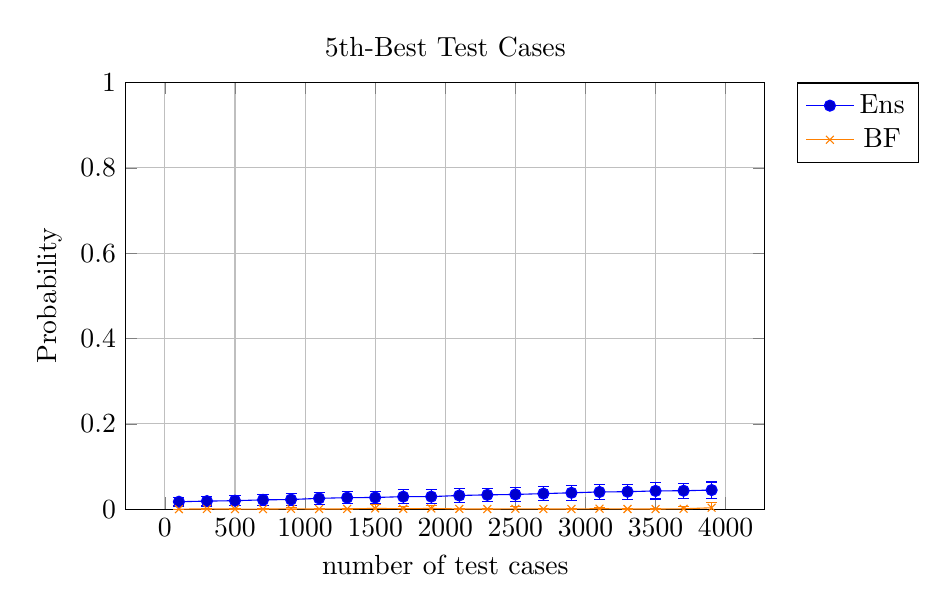
\begin{tikzpicture}
\begin{axis}[width=0.8\columnwidth,height=7cm,
  ymin=0,ymax=1,
  xtick={0,500,1000,1500,2000,2500,3000,3500,4000},
  xticklabels={0,500,1000,1500,2000,2500,3000,3500,4000},
  xlabel={number of test cases},ylabel={Probability},
  title={5th-Best Test Cases},grid=major,
  legend style={at={(1.05,1)},anchor=north west},
  error bars/y dir=both,error bars/y explicit]
\addplot+[mark=*,color=blue,error bars/.cd,y dir=both,y explicit] coordinates {
(100,0.01736000000000001) +- (0,0.010005631067615086)
(300,0.018840000000000013) +- (0,0.01141849555836172)
(500,0.01984000000000001) +- (0,0.012027790948550799)
(700,0.021740000000000002) +- (0,0.01339785240176917)
(900,0.022540000000000004) +- (0,0.014177029423165689)
(1100,0.02528000000000001) +- (0,0.013912320189717603)
(1300,0.026959999999999998) +- (0,0.014176669537788964)
(1500,0.027300000000000012) +- (0,0.014919169971987726)
(1700,0.029300000000000003) +- (0,0.01615770492896278)
(1900,0.029339999999999988) +- (0,0.01616952285590876)
(2100,0.03201999999999998) +- (0,0.016358845825262078)
(2300,0.033499999999999995) +- (0,0.015912067042060267)
(2500,0.03445999999999999) +- (0,0.016161443156412734)
(2700,0.036399999999999995) +- (0,0.016824423451928323)
(2900,0.03833999999999999) +- (0,0.017493567330855764)
(3100,0.040299999999999996) +- (0,0.017967374060007927)
(3300,0.040859999999999994) +- (0,0.01770738344791318)
(3500,0.04275999999999999) +- (0,0.019033332737648494)
(3700,0.04314) +- (0,0.01774077512514084)
(3900,0.044719999999999996) +- (0,0.018882061457848286)
};
\addlegendentry{Ens}
\addplot+[mark=x,color=orange,error bars/.cd,y dir=both,y explicit] coordinates {
(100,0.0) +- (0,0.0)
(300,0.0005800000000000001) +- (0,0.0015919440047582431)
(500,0.00014000000000000001) +- (0,0.0006064281507654607)
(700,0.0002) +- (0,0.0006060915267313264)
(900,0.00068) +- (0,0.002253704433476002)
(1100,0.00024) +- (0,0.0007159979477795239)
(1300,0.0005400000000000001) +- (0,0.0011466010106183494)
(1500,0.0017400000000000002) +- (0,0.00974534949269106)
(1700,0.0008799999999999999) +- (0,0.0052823927787876345)
(1900,0.0016) +- (0,0.0071997732390595166)
(2100,0.0005) +- (0,0.0017053337694733317)
(2300,0.00022000000000000006) +- (0,0.0009100347604933135)
(2500,0.0007400000000000001) +- (0,0.004530216015032521)
(2700,0.00044000000000000007) +- (0,0.0019183326093250876)
(2900,0.00036) +- (0,0.0012577920401745794)
(3100,0.0010400000000000001) +- (0,0.0035911455735756865)
(3300,0.00034) +- (0,0.0017215323027430405)
(3500,0.00024) +- (0,0.0008466018508588031)
(3700,0.0008600000000000001) +- (0,0.004973439658909749)
(3900,0.0032200000000000006) +- (0,0.012822636234409832)
};
\addlegendentry{BF}
\end{axis}
\end{tikzpicture}
\caption{BrokenPeterson (5th)}
\label{fig:BrokenPeterson_(5th)}
\end{figure}
\pgfplotsset{compat=1.3,width=0.8\columnwidth}
\begin{figure}[H]\centering\vspace{3ex}
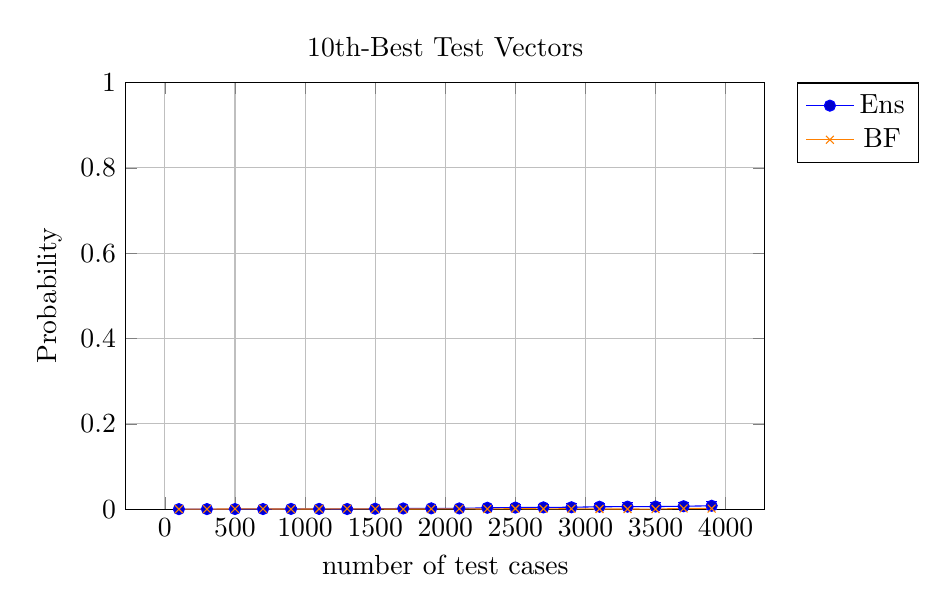
\begin{tikzpicture}
\begin{axis}[width=0.8\columnwidth,height=7cm,
  ymin=0,ymax=1,
  xtick={0,500,1000,1500,2000,2500,3000,3500,4000},
  xticklabels={0,500,1000,1500,2000,2500,3000,3500,4000},
  xlabel={number of test cases},ylabel={Probability},
  title={10th-Best Test Vectors},grid=major,
  legend style={at={(1.05,1)},anchor=north west},
  error bars/y dir=both,error bars/y explicit]
\addplot+[mark=*,color=blue,error bars/.cd,y dir=both,y explicit] coordinates {
(100,4e-05) +- (0,0.000282842712474619)
(300,0.00014000000000000001) +- (0,0.00040456577881446557)
(500,0.00021999999999999998) +- (0,0.0007082603003566023)
(700,0.00028000000000000003) +- (0,0.0008815570640309434)
(900,0.0005800000000000001) +- (0,0.002879129687093314)
(1100,0.0005800000000000002) +- (0,0.0013107094199987536)
(1300,0.0003000000000000001) +- (0,0.0007354021529276429)
(1500,0.0009600000000000003) +- (0,0.0025068070593192975)
(1700,0.00156) +- (0,0.002907836000203869)
(1900,0.0018800000000000004) +- (0,0.004618684325428529)
(2100,0.0016800000000000003) +- (0,0.0032226241050499487)
(2300,0.0032200000000000006) +- (0,0.005346331948740412)
(2500,0.0036200000000000004) +- (0,0.006803030537179435)
(2700,0.004140000000000001) +- (0,0.007392798481478788)
(2900,0.0044) +- (0,0.007835033829029765)
(3100,0.005640000000000002) +- (0,0.0080629158649274)
(3300,0.005860000000000001) +- (0,0.008771498371057786)
(3500,0.006100000000000003) +- (0,0.008493094433787044)
(3700,0.006800000000000003) +- (0,0.009516902257112264)
(3900,0.007900000000000003) +- (0,0.009540996396860124)
};
\addlegendentry{Ens}
\addplot+[mark=x,color=orange,error bars/.cd,y dir=both,y explicit] coordinates {
(100,0.0) +- (0,0.0)
(300,0.0) +- (0,0.0)
(500,0.00062) +- (0,0.0022304936764797893)
(700,0.00068) +- (0,0.0028098950521472563)
(900,2e-05) +- (0,0.00014142135623730954)
(1100,0.00058) +- (0,0.0017389886810019958)
(1300,0.0008) +- (0,0.0034699879432831767)
(1500,0.0006) +- (0,0.002175935173103974)
(1700,0.00018) +- (0,0.0008964783708421275)
(1900,0.0005) +- (0,0.0019086270308410552)
(2100,0.00072) +- (0,0.004384760249885915)
(2300,0.00028000000000000003) +- (0,0.0012128563015309213)
(2500,0.0011800000000000003) +- (0,0.003998418054528005)
(2700,0.00066) +- (0,0.003153294357671426)
(2900,0.0009200000000000001) +- (0,0.00231974664344965)
(3100,0.00034) +- (0,0.0012055991820481226)
(3300,0.00024) +- (0,0.001286666314194023)
(3500,0.00018) +- (0,0.0010038700623291924)
(3700,0.00166) +- (0,0.005783897421959962)
(3900,0.00136) +- (0,0.006579994417217407)
};
\addlegendentry{BF}
\end{axis}
\end{tikzpicture}
\caption{BrokenPeterson (10th)}
\label{fig:BrokenPeterson_(10th)}
\end{figure}
%----------------------------------------

\pgfplotsset{compat=1.3,width=0.8\columnwidth}
\begin{figure}[H]\centering\vspace{3ex}
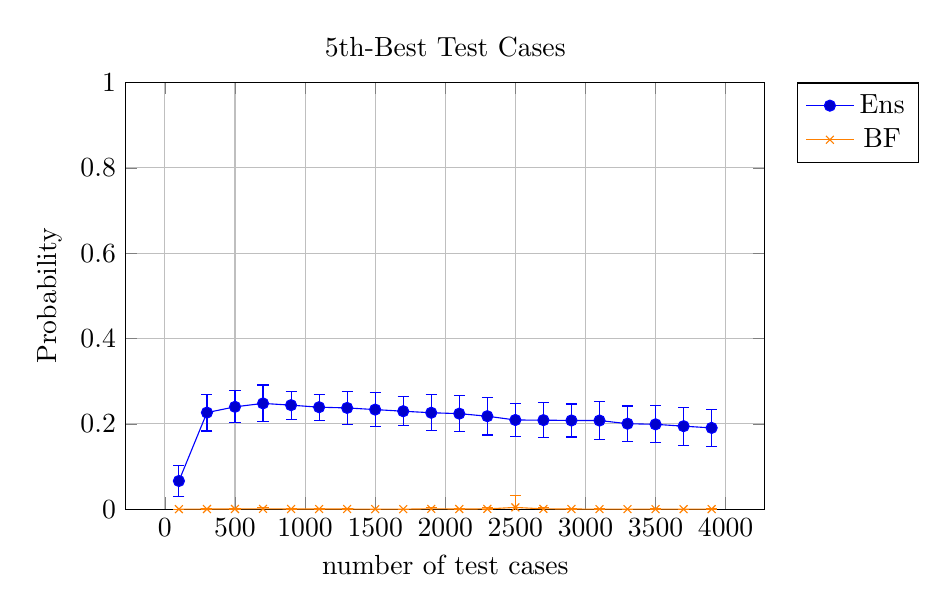
\begin{tikzpicture}
\begin{axis}[width=0.8\columnwidth,height=7cm,
  ymin=0,ymax=1,
  xtick={0,500,1000,1500,2000,2500,3000,3500,4000},
  xticklabels={0,500,1000,1500,2000,2500,3000,3500,4000},
  xlabel={number of test cases},ylabel={Probability},
  title={5th-Best Test Cases},grid=major,
  legend style={at={(1.05,1)},anchor=north west},
  error bars/y dir=both,error bars/y explicit]
\addplot+[mark=*,color=blue,error bars/.cd,y dir=both,y explicit] coordinates {
(100,0.066) +- (0,0.03589269722778876)
(300,0.22631999999999997) +- (0,0.04326965284287419)
(500,0.23980000000000004) +- (0,0.037438929864350226)
(700,0.24783999999999998) +- (0,0.04301179714773104)
(900,0.24372) +- (0,0.03283044878381867)
(1100,0.23892) +- (0,0.030119381515182734)
(1300,0.23723999999999998) +- (0,0.03912124533721681)
(1500,0.23334000000000002) +- (0,0.04006556361459412)
(1700,0.22950000000000004) +- (0,0.03446989221607368)
(1900,0.22594000000000006) +- (0,0.041967630869711024)
(2100,0.22384000000000004) +- (0,0.041956906950063655)
(2300,0.21782000000000004) +- (0,0.04399939238912546)
(2500,0.20894000000000001) +- (0,0.038761126118305275)
(2700,0.20858000000000002) +- (0,0.04061672019235024)
(2900,0.20783999999999994) +- (0,0.03872791536568211)
(3100,0.20768) +- (0,0.04504212993840045)
(3300,0.20028) +- (0,0.04153240190698436)
(3500,0.19879999999999998) +- (0,0.04340553900513773)
(3700,0.19444000000000006) +- (0,0.04425075117545243)
(3900,0.19044) +- (0,0.04264143811948615)
};
\addlegendentry{Ens}
\addplot+[mark=x,color=orange,error bars/.cd,y dir=both,y explicit] coordinates {
(100,0.0) +- (0,0.0)
(300,0.00028000000000000003) +- (0,0.0009267014137272489)
(500,0.00042) +- (0,0.0016913947873073904)
(700,0.00074) +- (0,0.0032938408818736285)
(900,0.00033999999999999997) +- (0,0.0015985963230539574)
(1100,0.00020000000000000004) +- (0,0.0007559289460184544)
(1300,0.00028) +- (0,0.0016040764397277942)
(1500,0.0) +- (0,0.0)
(1700,0.0) +- (0,0.0)
(1900,0.00072) +- (0,0.0036029466398762996)
(2100,0.00028000000000000003) +- (0,0.0017147618386427037)
(2300,0.0005600000000000001) +- (0,0.002612059942431862)
(2500,0.00408) +- (0,0.028132224242251567)
(2700,0.00058) +- (0,0.003823077081010392)
(2900,0.0003) +- (0,0.0017172593257387583)
(3100,6e-05) +- (0,0.00023989793748209517)
(3300,2e-05) +- (0,0.00014142135623730954)
(3500,6e-05) +- (0,0.0004242640687119285)
(3700,2e-05) +- (0,0.0001414213562373096)
(3900,0.0001) +- (0,0.00041649656391752143)
};
\addlegendentry{BF}
\end{axis}
\end{tikzpicture}
\caption{DelayedWrite (5th)}
\label{fig:DelayedWrite_(5th)}
\end{figure}
\pgfplotsset{compat=1.3,width=0.8\columnwidth}
\begin{figure}[H]\centering\vspace{3ex}
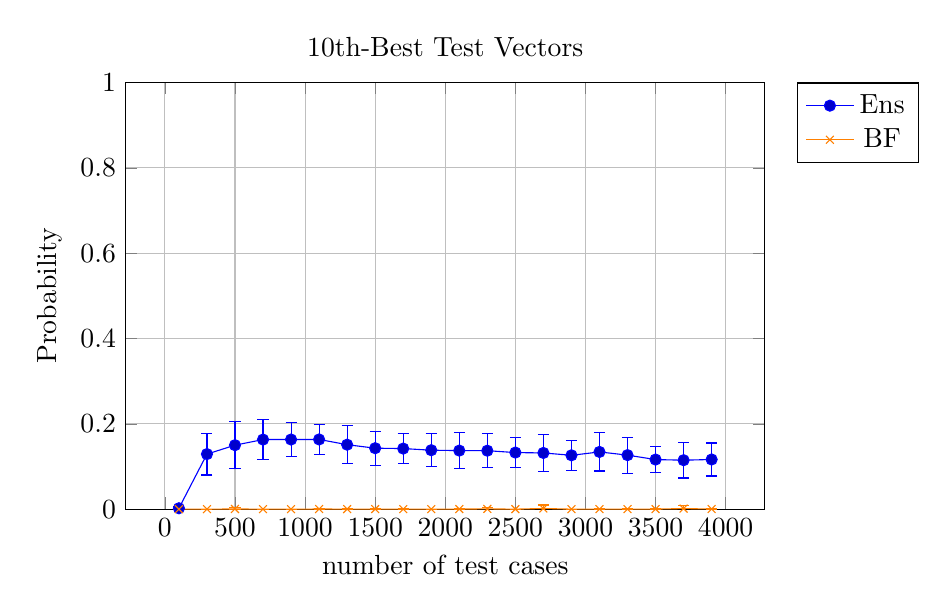
\begin{tikzpicture}
\begin{axis}[width=0.8\columnwidth,height=7cm,
  ymin=0,ymax=1,
  xtick={0,500,1000,1500,2000,2500,3000,3500,4000},
  xticklabels={0,500,1000,1500,2000,2500,3000,3500,4000},
  xlabel={number of test cases},ylabel={Probability},
  title={10th-Best Test Vectors},grid=major,
  legend style={at={(1.05,1)},anchor=north west},
  error bars/y dir=both,error bars/y explicit]
\addplot+[mark=*,color=blue,error bars/.cd,y dir=both,y explicit] coordinates {
(100,0.0020599999999999998) +- (0,0.0033951345739911707)
(300,0.12904) +- (0,0.049078845353415626)
(500,0.14994000000000005) +- (0,0.055172978449784596)
(700,0.1631) +- (0,0.04727697372821109)
(900,0.16319999999999996) +- (0,0.038928505897717056)
(1100,0.16335999999999995) +- (0,0.03435157959116563)
(1300,0.15108000000000008) +- (0,0.04456082291402936)
(1500,0.14286000000000004) +- (0,0.039705554024697255)
(1700,0.14198) +- (0,0.03566653379083898)
(1900,0.13816) +- (0,0.03906423804296655)
(2100,0.13723999999999997) +- (0,0.04153707957466244)
(2300,0.137) +- (0,0.03993770659618884)
(2500,0.13261999999999996) +- (0,0.03539508209814896)
(2700,0.13174) +- (0,0.043100172829806466)
(2900,0.12618000000000001) +- (0,0.035019347422211376)
(3100,0.13409999999999997) +- (0,0.04471964824073995)
(3300,0.12658000000000005) +- (0,0.04230023399365956)
(3500,0.11622000000000002) +- (0,0.03062697890316125)
(3700,0.11472000000000002) +- (0,0.04162222718594428)
(3900,0.11639999999999998) +- (0,0.03859364439587311)
};
\addlegendentry{Ens}
\addplot+[mark=x,color=orange,error bars/.cd,y dir=both,y explicit] coordinates {
(100,0.0) +- (0,0.0)
(300,0.0) +- (0,0.0)
(500,0.0004000000000000001) +- (0,0.002415933503612538)
(700,2e-05) +- (0,0.00014142135623730954)
(900,0.0) +- (0,0.0)
(1100,0.00028000000000000003) +- (0,0.0013856406460551018)
(1300,0.00014000000000000001) +- (0,0.0009899494936611666)
(1500,0.00018) +- (0,0.00102399776785471)
(1700,8e-05) +- (0,0.00044446711960297275)
(1900,2e-05) +- (0,0.0001414213562373096)
(2100,0.00024) +- (0,0.0012047524938461722)
(2300,0.0006) +- (0,0.002969229955832361)
(2500,0.0) +- (0,0.0)
(2700,0.00154) +- (0,0.008094366899900453)
(2900,0.0) +- (0,0.0)
(3100,0.00016) +- (0,0.0006502746672423452)
(3300,0.00018) +- (0,0.0008964783708421275)
(3500,0.00018) +- (0,0.001137307956428294)
(3700,0.0013) +- (0,0.006231093853589826)
(3900,0.00030000000000000003) +- (0,0.0010738068841694935)
};
\addlegendentry{BF}
\end{axis}
\end{tikzpicture}
\caption{DelayedWrite (10th)}
\label{fig:DelayedWrite_(10th)}
\end{figure}
%----------------------------------------

\pgfplotsset{compat=1.3,width=0.8\columnwidth}
\begin{figure}[H]\centering\vspace{3ex}
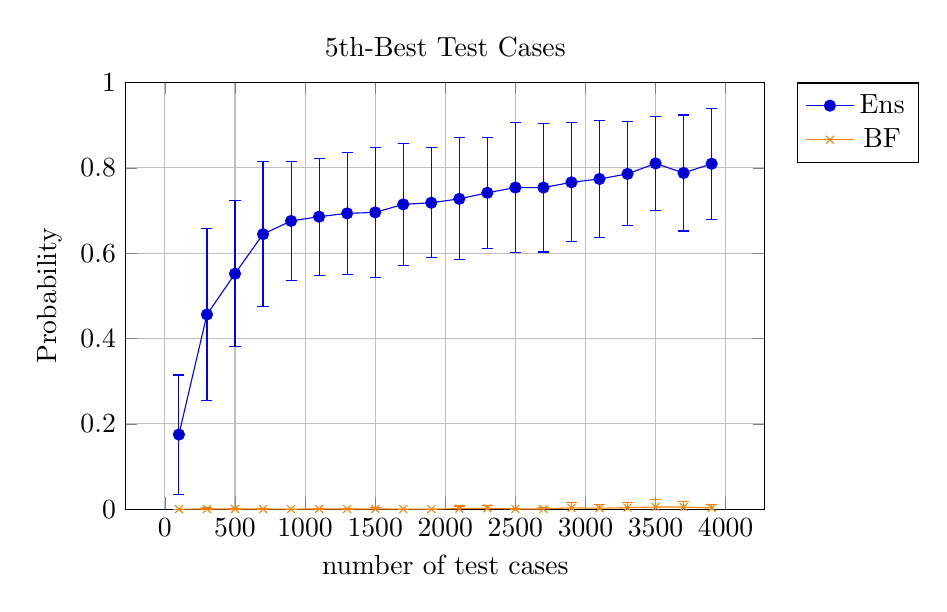
\begin{tikzpicture}
\begin{axis}[width=0.8\columnwidth,height=7cm,
  ymin=0,ymax=1,
  xtick={0,500,1000,1500,2000,2500,3000,3500,4000},
  xticklabels={0,500,1000,1500,2000,2500,3000,3500,4000},
  xlabel={number of test cases},ylabel={Probability},
  title={5th-Best Test Cases},grid=major,
  legend style={at={(1.05,1)},anchor=north west},
  error bars/y dir=both,error bars/y explicit]
\addplot+[mark=*,color=blue,error bars/.cd,y dir=both,y explicit] coordinates {
(100,0.17481999999999995) +- (0,0.13955639486221616)
(300,0.4562600000000001) +- (0,0.20106896065473479)
(500,0.5517999999999998) +- (0,0.17145475990440648)
(700,0.6445800000000002) +- (0,0.1692658927515498)
(900,0.6754599999999997) +- (0,0.13919758530629198)
(1100,0.6855) +- (0,0.13717488465310185)
(1300,0.69324) +- (0,0.1425918336385649)
(1500,0.6955599999999998) +- (0,0.15245182042540723)
(1700,0.7143599999999998) +- (0,0.14225082188349958)
(1900,0.7181199999999999) +- (0,0.12902770466620186)
(2100,0.72726) +- (0,0.1428615442179124)
(2300,0.7415) +- (0,0.13002374194503022)
(2500,0.75374) +- (0,0.1525172201719523)
(2700,0.75366) +- (0,0.1509816328875392)
(2900,0.7660399999999999) +- (0,0.13975561176714263)
(3100,0.7739) +- (0,0.1366612451222645)
(3300,0.7857999999999998) +- (0,0.12174831851497825)
(3500,0.8103200000000003) +- (0,0.11081634742736612)
(3700,0.7878799999999998) +- (0,0.1359101804239011)
(3900,0.8095799999999999) +- (0,0.1301053089945675)
};
\addlegendentry{Ens}
\addplot+[mark=x,color=orange,error bars/.cd,y dir=both,y explicit] coordinates {
(100,0.0) +- (0,0.0)
(300,0.00043999999999999996) +- (0,0.0021396165973541774)
(500,0.00032) +- (0,0.0012525891552447412)
(700,0.0003) +- (0,0.0012330483215451478)
(900,0.0) +- (0,0.0)
(1100,0.0005200000000000001) +- (0,0.0019403344967256736)
(1300,0.00020000000000000004) +- (0,0.0006388765649999399)
(1500,0.00046) +- (0,0.002851494416645992)
(1700,0.0) +- (0,0.0)
(1900,0.0) +- (0,0.0)
(2100,0.0011) +- (0,0.006181770435262516)
(2300,0.00188) +- (0,0.007319640896734133)
(2500,0.00032) +- (0,0.0016956125857094616)
(2700,0.00042) +- (0,0.0028290764339953343)
(2900,0.00302) +- (0,0.011920638936443852)
(3100,0.00216) +- (0,0.009564731132271994)
(3300,0.003560000000000001) +- (0,0.011469854010422633)
(3500,0.00496) +- (0,0.01733459440729163)
(3700,0.004940000000000001) +- (0,0.012784572973801235)
(3900,0.0029000000000000002) +- (0,0.008662021256317601)
};
\addlegendentry{BF}
\end{axis}
\end{tikzpicture}
\caption{IfNotWhile (5th)}
\label{fig:IfNotWhile_(5th)}
\end{figure}
\pgfplotsset{compat=1.3,width=0.8\columnwidth}
\begin{figure}[H]\centering\vspace{3ex}
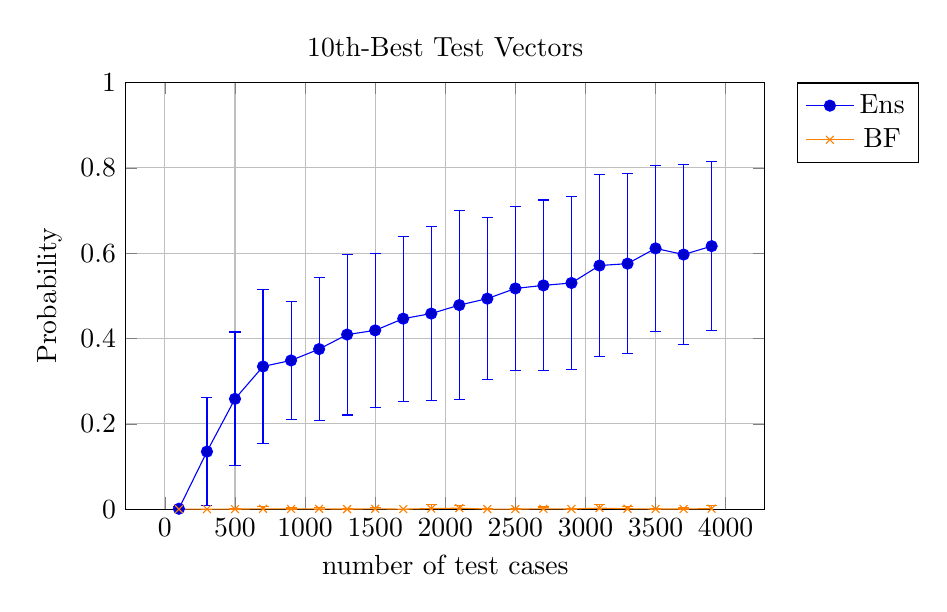
\begin{tikzpicture}
\begin{axis}[width=0.8\columnwidth,height=7cm,
  ymin=0,ymax=1,
  xtick={0,500,1000,1500,2000,2500,3000,3500,4000},
  xticklabels={0,500,1000,1500,2000,2500,3000,3500,4000},
  xlabel={number of test cases},ylabel={Probability},
  title={10th-Best Test Vectors},grid=major,
  legend style={at={(1.05,1)},anchor=north west},
  error bars/y dir=both,error bars/y explicit]
\addplot+[mark=*,color=blue,error bars/.cd,y dir=both,y explicit] coordinates {
(100,0.00094) +- (0,0.004316130163912661)
(300,0.13488) +- (0,0.1260860800875209)
(500,0.25848000000000004) +- (0,0.15668846512121049)
(700,0.33444000000000007) +- (0,0.18131944524647578)
(900,0.3485400000000001) +- (0,0.13806626773297737)
(1100,0.37515999999999994) +- (0,0.16809950406026242)
(1300,0.4092) +- (0,0.18861114300408158)
(1500,0.4189799999999999) +- (0,0.18096447841767097)
(1700,0.4464799999999999) +- (0,0.1932052139407153)
(1900,0.4583599999999998) +- (0,0.20392783437445003)
(2100,0.47826) +- (0,0.22200696900258424)
(2300,0.49337999999999993) +- (0,0.19001062161503157)
(2500,0.5173) +- (0,0.19219550526715776)
(2700,0.5244199999999999) +- (0,0.20023976342660538)
(2900,0.53006) +- (0,0.20348949829995494)
(3100,0.5709599999999999) +- (0,0.21269494875170375)
(3300,0.57538) +- (0,0.2111273810295772)
(3500,0.6112) +- (0,0.19421133029853466)
(3700,0.5966600000000001) +- (0,0.21118457059440396)
(3900,0.61646) +- (0,0.19796579894269706)
};
\addlegendentry{Ens}
\addplot+[mark=x,color=orange,error bars/.cd,y dir=both,y explicit] coordinates {
(100,0.0) +- (0,0.0)
(300,0.0) +- (0,0.0)
(500,0.0001) +- (0,0.0005802884574739973)
(700,0.0008) +- (0,0.005371884479132333)
(900,0.0004000000000000001) +- (0,0.0022857142857142855)
(1100,0.0007400000000000001) +- (0,0.002776063870346808)
(1300,8e-05) +- (0,0.000565685424949238)
(1500,0.0007599999999999999) +- (0,0.003359786193391794)
(1700,2e-05) +- (0,0.0001414213562373096)
(1900,0.00136) +- (0,0.008625448820028948)
(2100,0.00224) +- (0,0.006799039548017808)
(2300,0.00014000000000000001) +- (0,0.0005717856027482714)
(2500,0.00012) +- (0,0.0005205962045225313)
(2700,0.00082) +- (0,0.004084265477389529)
(2900,0.00032) +- (0,0.00164676553725595)
(3100,0.00234) +- (0,0.00809285399066891)
(3300,0.0009400000000000002) +- (0,0.004330291973000039)
(3500,0.00028) +- (0,0.0013856406460551018)
(3700,0.0005) +- (0,0.0022154374884672604)
(3900,0.0011) +- (0,0.0069259936294442295)
};
\addlegendentry{BF}
\end{axis}
\end{tikzpicture}
\caption{IfNotWhile (10th)}
\label{fig:IfNotWhile_(10th)}
\end{figure}
%----------------------------------------

\pgfplotsset{compat=1.3,width=0.8\columnwidth}
\begin{figure}[H]\centering\vspace{3ex}
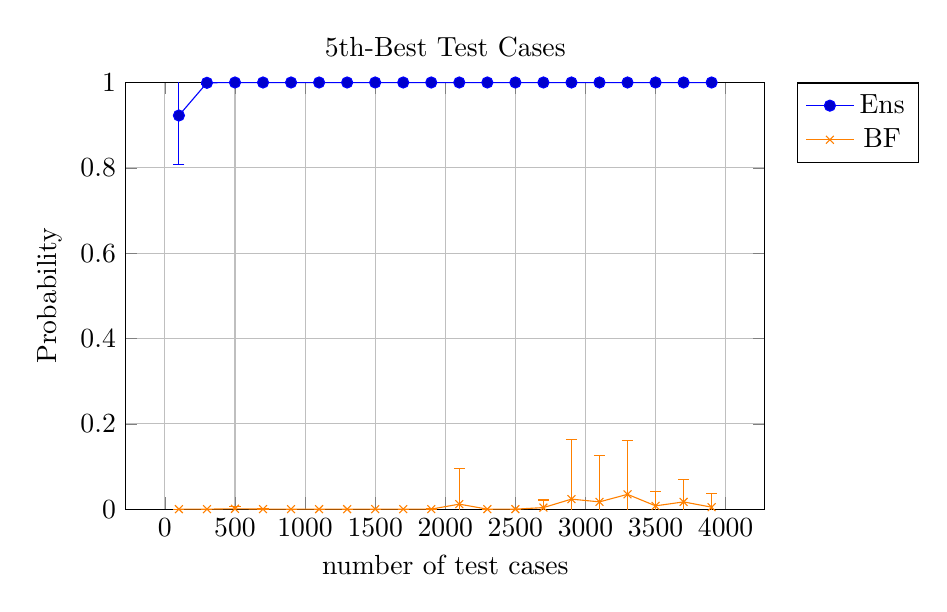
\begin{tikzpicture}
\begin{axis}[width=0.8\columnwidth,height=7cm,
  ymin=0,ymax=1,
  xtick={0,500,1000,1500,2000,2500,3000,3500,4000},
  xticklabels={0,500,1000,1500,2000,2500,3000,3500,4000},
  xlabel={number of test cases},ylabel={Probability},
  title={5th-Best Test Cases},grid=major,
  legend style={at={(1.05,1)},anchor=north west},
  error bars/y dir=both,error bars/y explicit]
\addplot+[mark=*,color=blue,error bars/.cd,y dir=both,y explicit] coordinates {
(100,0.9226400000000001) +- (0,0.11543065061776688)
(300,0.99924) +- (0,0.004951025455521777)
(500,1.0) +- (0,0.0)
(700,1.0) +- (0,0.0)
(900,1.0) +- (0,0.0)
(1100,1.0) +- (0,0.0)
(1300,1.0) +- (0,0.0)
(1500,1.0) +- (0,0.0)
(1700,1.0) +- (0,0.0)
(1900,1.0) +- (0,0.0)
(2100,1.0) +- (0,0.0)
(2300,1.0) +- (0,0.0)
(2500,1.0) +- (0,0.0)
(2700,1.0) +- (0,0.0)
(2900,1.0) +- (0,0.0)
(3100,1.0) +- (0,0.0)
(3300,1.0) +- (0,0.0)
(3500,1.0) +- (0,0.0)
(3700,1.0) +- (0,0.0)
(3900,1.0) +- (0,0.0)
};
\addlegendentry{Ens}
\addplot+[mark=x,color=orange,error bars/.cd,y dir=both,y explicit] coordinates {
(100,0.0) +- (0,0.0)
(300,0.0) +- (0,0.0)
(500,0.00082) +- (0,0.00579827560572969)
(700,0.0001) +- (0,0.0005050762722761054)
(900,0.0) +- (0,0.0)
(1100,0.0) +- (0,0.0)
(1300,0.0) +- (0,0.0)
(1500,0.0) +- (0,0.0)
(1700,0.0) +- (0,0.0)
(1900,0.0001) +- (0,0.0007071067811865476)
(2100,0.01172) +- (0,0.08287291475506338)
(2300,0.0) +- (0,0.0)
(2500,0.0) +- (0,0.0)
(2700,0.00362) +- (0,0.017916917099974172)
(2900,0.023479999999999997) +- (0,0.13926721342331036)
(3100,0.01704) +- (0,0.10796691859178015)
(3300,0.0347) +- (0,0.126729222827126)
(3500,0.007719999999999999) +- (0,0.033823696559950274)
(3700,0.016980000000000006) +- (0,0.05183863896550447)
(3900,0.0046) +- (0,0.03252691193458118)
};
\addlegendentry{BF}
\end{axis}
\end{tikzpicture}
\caption{LockOrderInversion (5th)}
\label{fig:LockOrderInversion_(5th)}
\end{figure}
\pgfplotsset{compat=1.3,width=0.8\columnwidth}
\begin{figure}[H]\centering\vspace{3ex}
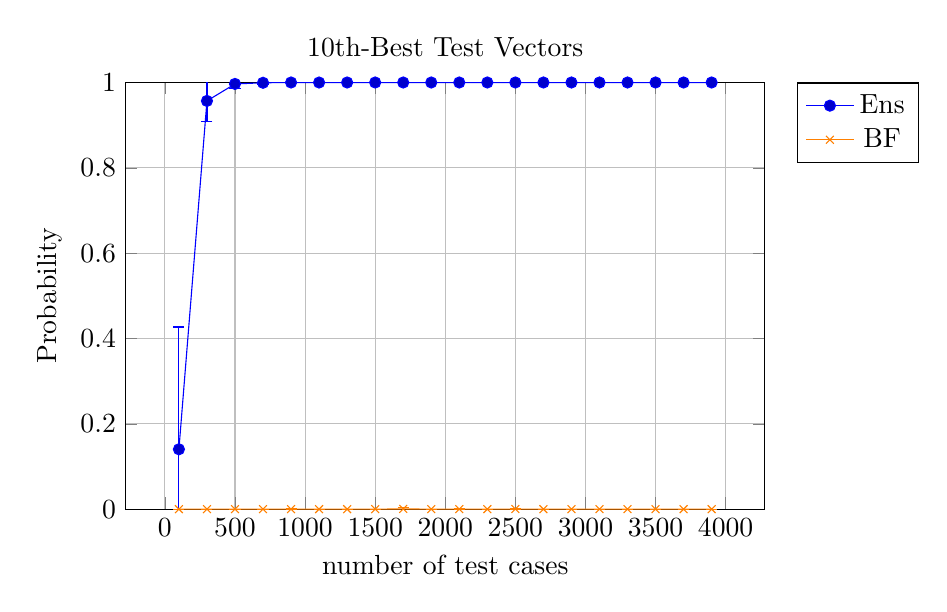
\begin{tikzpicture}
\begin{axis}[width=0.8\columnwidth,height=7cm,
  ymin=0,ymax=1,
  xtick={0,500,1000,1500,2000,2500,3000,3500,4000},
  xticklabels={0,500,1000,1500,2000,2500,3000,3500,4000},
  xlabel={number of test cases},ylabel={Probability},
  title={10th-Best Test Vectors},grid=major,
  legend style={at={(1.05,1)},anchor=north west},
  error bars/y dir=both,error bars/y explicit]
\addplot+[mark=*,color=blue,error bars/.cd,y dir=both,y explicit] coordinates {
(100,0.14029999999999998) +- (0,0.28658803897167917)
(300,0.9568199999999999) +- (0,0.0487457753271491)
(500,0.99664) +- (0,0.009993385567566229)
(700,0.99932) +- (0,0.00480832611206853)
(900,1.0) +- (0,0.0)
(1100,0.99994) +- (0,0.00042426406871192926)
(1300,1.0) +- (0,0.0)
(1500,1.0) +- (0,0.0)
(1700,1.0) +- (0,0.0)
(1900,1.0) +- (0,0.0)
(2100,1.0) +- (0,0.0)
(2300,1.0) +- (0,0.0)
(2500,1.0) +- (0,0.0)
(2700,1.0) +- (0,0.0)
(2900,1.0) +- (0,0.0)
(3100,1.0) +- (0,0.0)
(3300,1.0) +- (0,0.0)
(3500,1.0) +- (0,0.0)
(3700,1.0) +- (0,0.0)
(3900,1.0) +- (0,0.0)
};
\addlegendentry{Ens}
\addplot+[mark=x,color=orange,error bars/.cd,y dir=both,y explicit] coordinates {
(100,0.0) +- (0,0.0)
(300,0.0) +- (0,0.0)
(500,0.0) +- (0,0.0)
(700,0.0) +- (0,0.0)
(900,6e-05) +- (0,0.0004242640687119285)
(1100,0.0) +- (0,0.0)
(1300,0.0) +- (0,0.0)
(1500,0.0) +- (0,0.0)
(1700,0.0005) +- (0,0.003535533905932738)
(1900,0.0) +- (0,0.0)
(2100,0.00012) +- (0,0.000848528137423857)
(2300,0.0) +- (0,0.0)
(2500,0.00024) +- (0,0.001697056274847714)
(2700,0.0) +- (0,0.0)
(2900,0.0) +- (0,0.0)
(3100,0.0) +- (0,0.0)
(3300,0.0) +- (0,0.0)
(3500,0.0) +- (0,0.0)
(3700,0.0) +- (0,0.0)
(3900,0.0) +- (0,0.0)
};
\addlegendentry{BF}
\end{axis}
\end{tikzpicture}
\caption{LockOrderInversion (10th)}
\label{fig:LockOrderInversion_(10th)}
\end{figure}
%----------------------------------------

\pgfplotsset{compat=1.3,width=0.8\columnwidth}
\begin{figure}[H]\centering\vspace{3ex}
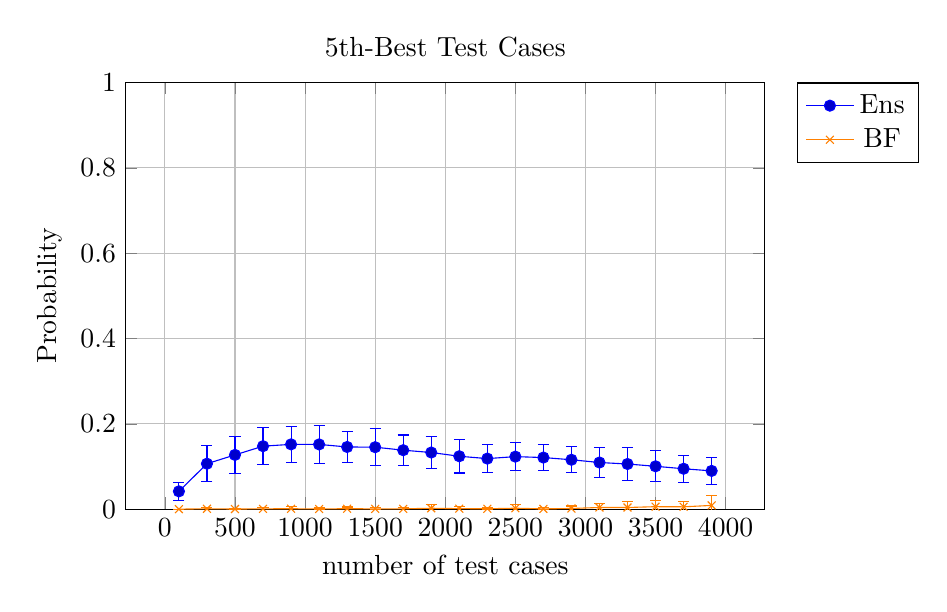
\begin{tikzpicture}
\begin{axis}[width=0.8\columnwidth,height=7cm,
  ymin=0,ymax=1,
  xtick={0,500,1000,1500,2000,2500,3000,3500,4000},
  xticklabels={0,500,1000,1500,2000,2500,3000,3500,4000},
  xlabel={number of test cases},ylabel={Probability},
  title={5th-Best Test Cases},grid=major,
  legend style={at={(1.05,1)},anchor=north west},
  error bars/y dir=both,error bars/y explicit]
\addplot+[mark=*,color=blue,error bars/.cd,y dir=both,y explicit] coordinates {
(100,0.0417) +- (0,0.021765212835989426)
(300,0.10648000000000003) +- (0,0.04177258157486278)
(500,0.12714000000000003) +- (0,0.043990727223275586)
(700,0.14758000000000002) +- (0,0.04298224123082104)
(900,0.15184000000000003) +- (0,0.042426099014062184)
(1100,0.15171999999999997) +- (0,0.04486171041349748)
(1300,0.14574) +- (0,0.03718009671634458)
(1500,0.1452) +- (0,0.042955126086916054)
(1700,0.13817999999999997) +- (0,0.035647760899429067)
(1900,0.13274) +- (0,0.037430103567332354)
(2100,0.12396000000000001) +- (0,0.039145964423069744)
(2300,0.11845999999999998) +- (0,0.03283304084955545)
(2500,0.12309999999999999) +- (0,0.033038783641196535)
(2700,0.12092000000000006) +- (0,0.03131592800698654)
(2900,0.11574000000000001) +- (0,0.03014171290990035)
(3100,0.1093) +- (0,0.03583935244495176)
(3300,0.10582000000000003) +- (0,0.03820443931892553)
(3500,0.10039999999999999) +- (0,0.03649098295106204)
(3700,0.09470000000000002) +- (0,0.03183583528295216)
(3900,0.08963999999999998) +- (0,0.030940865257085927)
};
\addlegendentry{Ens}
\addplot+[mark=x,color=orange,error bars/.cd,y dir=both,y explicit] coordinates {
(100,0.0) +- (0,0.0)
(300,0.0008800000000000001) +- (0,0.003645741155297311)
(500,0.00028) +- (0,0.0012623269733928297)
(700,0.00072) +- (0,0.0030307269956973987)
(900,0.00094) +- (0,0.004239801689624992)
(1100,0.0003800000000000001) +- (0,0.0022757819916392227)
(1300,0.00104) +- (0,0.003969064044300003)
(1500,0.0006199999999999999) +- (0,0.0022757819916392227)
(1700,0.0007400000000000001) +- (0,0.0036073055125986336)
(1900,0.0020800000000000003) +- (0,0.008930205564743257)
(2100,0.00116) +- (0,0.0049088009259504765)
(2300,0.0008800000000000001) +- (0,0.0027894846279906114)
(2500,0.00218) +- (0,0.008800950783516379)
(2700,0.00062) +- (0,0.0022213252157857735)
(2900,0.00154) +- (0,0.0058176718816420865)
(3100,0.003920000000000001) +- (0,0.008782728877211925)
(3300,0.00386) +- (0,0.013173891929548709)
(3500,0.00578) +- (0,0.014585833216249419)
(3700,0.005460000000000001) +- (0,0.012005457942459474)
(3900,0.00876) +- (0,0.02299117843248331)
};
\addlegendentry{BF}
\end{axis}
\end{tikzpicture}
\caption{LostSignal (5th)}
\label{fig:LostSignal_(5th)}
\end{figure}
\pgfplotsset{compat=1.3,width=0.8\columnwidth}
\begin{figure}[H]\centering\vspace{3ex}
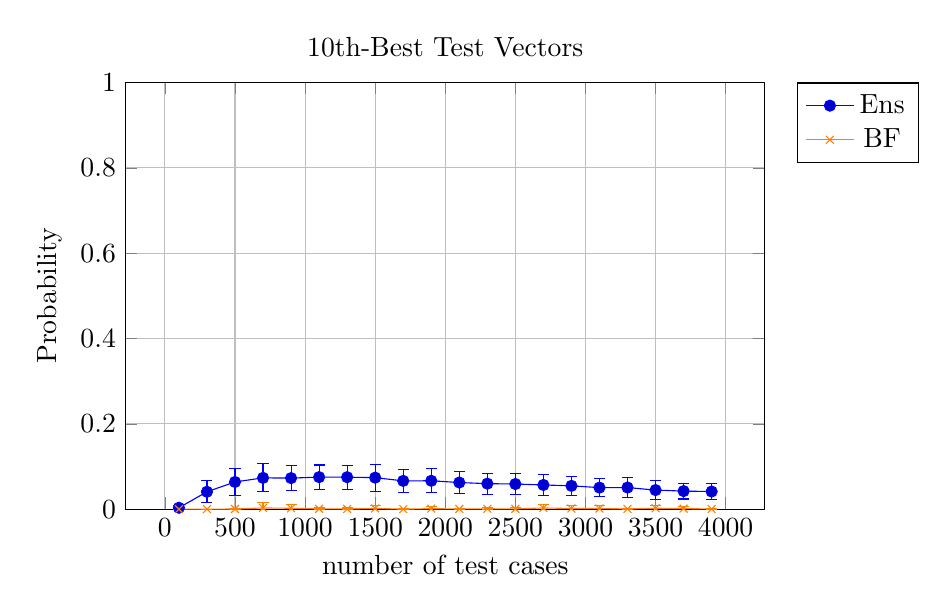
\begin{tikzpicture}
\begin{axis}[width=0.8\columnwidth,height=7cm,
  ymin=0,ymax=1,
  xtick={0,500,1000,1500,2000,2500,3000,3500,4000},
  xticklabels={0,500,1000,1500,2000,2500,3000,3500,4000},
  xlabel={number of test cases},ylabel={Probability},
  title={10th-Best Test Vectors},grid=major,
  legend style={at={(1.05,1)},anchor=north west},
  error bars/y dir=both,error bars/y explicit]
\addplot+[mark=*,color=blue,error bars/.cd,y dir=both,y explicit] coordinates {
(100,0.0032000000000000006) +- (0,0.0045039665058384136)
(300,0.04074) +- (0,0.026037500428640024)
(500,0.06369999999999999) +- (0,0.03213825363859673)
(700,0.07329999999999999) +- (0,0.03264918663236653)
(900,0.07278000000000003) +- (0,0.029727531388411284)
(1100,0.07504) +- (0,0.028357024109143265)
(1300,0.07490000000000002) +- (0,0.02821365279579426)
(1500,0.07382000000000001) +- (0,0.03159158374101091)
(1700,0.06624000000000001) +- (0,0.026225521142270412)
(1900,0.06649999999999999) +- (0,0.02824401688492487)
(2100,0.06238) +- (0,0.02620709516017933)
(2300,0.05973999999999999) +- (0,0.024621883414092115)
(2500,0.05887999999999999) +- (0,0.02413621210326673)
(2700,0.05668) +- (0,0.025324377221022678)
(2900,0.05466) +- (0,0.022871076110427744)
(3100,0.05041999999999999) +- (0,0.02050096065444501)
(3300,0.05062000000000001) +- (0,0.02380609594372062)
(3500,0.04465999999999999) +- (0,0.022985896296891052)
(3700,0.0423) +- (0,0.01844711138274358)
(3900,0.04130000000000001) +- (0,0.01831610198259263)
};
\addlegendentry{Ens}
\addplot+[mark=x,color=orange,error bars/.cd,y dir=both,y explicit] coordinates {
(100,0.0) +- (0,0.0)
(300,0.0) +- (0,0.0)
(500,0.00032) +- (0,0.0012195683411664595)
(700,0.0028200000000000005) +- (0,0.01357171428270683)
(900,0.00202) +- (0,0.0080317990461893)
(1100,0.00064) +- (0,0.0019770107305149935)
(1300,0.0005399999999999999) +- (0,0.002022425296922646)
(1500,0.0016600000000000005) +- (0,0.0063619083262037345)
(1700,4e-05) +- (0,0.000282842712474619)
(1900,0.0011200000000000001) +- (0,0.005220211896551514)
(2100,0.00042000000000000007) +- (0,0.0018745339556861611)
(2300,0.0008399999999999999) +- (0,0.0028739505626810447)
(2500,0.00068) +- (0,0.0032666527835329036)
(2700,0.0027800000000000004) +- (0,0.008079427136693719)
(2900,0.00154) +- (0,0.006487696361701329)
(3100,0.0014200000000000003) +- (0,0.007045305282996065)
(3300,0.0005200000000000001) +- (0,0.0019085201019616838)
(3500,0.00214) +- (0,0.006446039758753321)
(3700,0.00134) +- (0,0.004033583508292266)
(3900,0.00037999999999999997) +- (0,0.001872355277642116)
};
\addlegendentry{BF}
\end{axis}
\end{tikzpicture}
\caption{LostSignal (10th)}
\label{fig:LostSignal_(10th)}
\end{figure}
%----------------------------------------

\pgfplotsset{compat=1.3,width=0.8\columnwidth}
\begin{figure}[H]\centering\vspace{3ex}
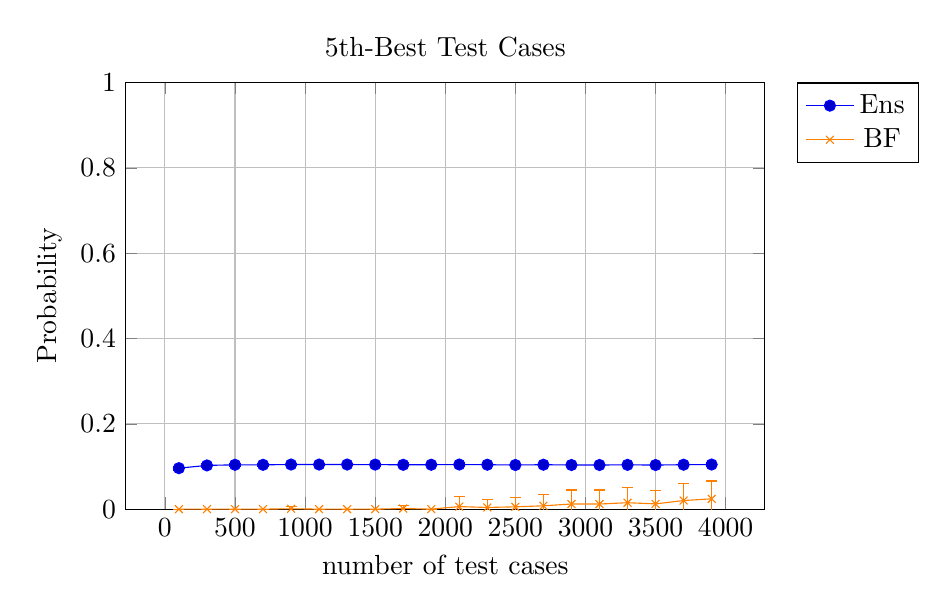
\begin{tikzpicture}
\begin{axis}[width=0.8\columnwidth,height=7cm,
  ymin=0,ymax=1,
  xtick={0,500,1000,1500,2000,2500,3000,3500,4000},
  xticklabels={0,500,1000,1500,2000,2500,3000,3500,4000},
  xlabel={number of test cases},ylabel={Probability},
  title={5th-Best Test Cases},grid=major,
  legend style={at={(1.05,1)},anchor=north west},
  error bars/y dir=both,error bars/y explicit]
\addplot+[mark=*,color=blue,error bars/.cd,y dir=both,y explicit] coordinates {
(100,0.09606000000000003) +- (0,0.004210821820994482)
(300,0.10250000000000004) +- (0,0.004450406998127203)
(500,0.10392000000000001) +- (0,0.0028702556239712813)
(700,0.10390000000000002) +- (0,0.003465574134488057)
(900,0.10458000000000002) +- (0,0.0029972095866192677)
(1100,0.10450000000000002) +- (0,0.0029846546308251692)
(1300,0.10456000000000004) +- (0,0.0032145079288267106)
(1500,0.10438) +- (0,0.003306703148800284)
(1700,0.10394000000000003) +- (0,0.004353792622999129)
(1900,0.10410000000000005) +- (0,0.002704870889823069)
(2100,0.10456000000000003) +- (0,0.0036374469629347535)
(2300,0.10412000000000005) +- (0,0.00380997616361926)
(2500,0.10346000000000004) +- (0,0.0034417010507086423)
(2700,0.10414000000000001) +- (0,0.003295079820035953)
(2900,0.10348000000000004) +- (0,0.00290839741270069)
(3100,0.10346000000000004) +- (0,0.0031957241841599035)
(3300,0.10384) +- (0,0.003012626489850166)
(3500,0.10336000000000004) +- (0,0.0025774532597357485)
(3700,0.10414000000000004) +- (0,0.0031752229553728235)
(3900,0.10458000000000002) +- (0,0.0037147801868663345)
};
\addlegendentry{Ens}
\addplot+[mark=x,color=orange,error bars/.cd,y dir=both,y explicit] coordinates {
(100,0.0) +- (0,0.0)
(300,0.0) +- (0,0.0)
(500,2e-05) +- (0,0.0001414213562373096)
(700,0.0) +- (0,0.0)
(900,0.00086) +- (0,0.006081118318204308)
(1100,0.0) +- (0,0.0)
(1300,0.0) +- (0,0.0)
(1500,0.0) +- (0,0.0)
(1700,0.0014000000000000002) +- (0,0.007561988724494885)
(1900,0.0) +- (0,0.0)
(2100,0.00598) +- (0,0.02399021058852199)
(2300,0.00396) +- (0,0.01964787987731677)
(2500,0.005399999999999999) +- (0,0.021721803209997954)
(2700,0.00786) +- (0,0.026951210642604553)
(2900,0.012) +- (0,0.03283415344809519)
(3100,0.012) +- (0,0.032747643629203405)
(3300,0.015059999999999997) +- (0,0.03543053565983525)
(3500,0.0123) +- (0,0.03096756038047504)
(3700,0.0202) +- (0,0.03979539507766891)
(3900,0.02418) +- (0,0.041690643985411974)
};
\addlegendentry{BF}
\end{axis}
\end{tikzpicture}
\caption{PartialLock (5th)}
\label{fig:PartialLock_(5th)}
\end{figure}
\pgfplotsset{compat=1.3,width=0.8\columnwidth}
\begin{figure}[H]\centering\vspace{3ex}
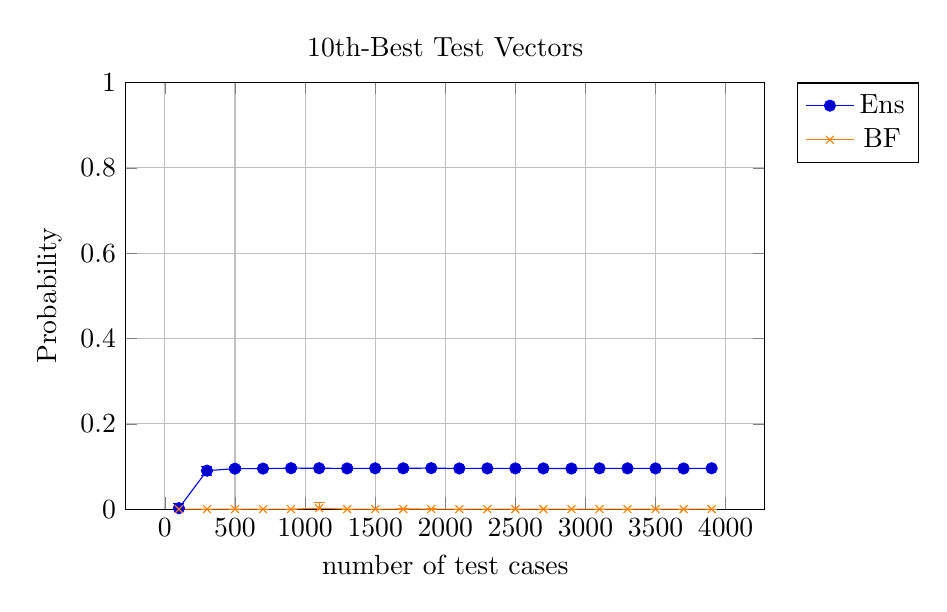
\begin{tikzpicture}
\begin{axis}[width=0.8\columnwidth,height=7cm,
  ymin=0,ymax=1,
  xtick={0,500,1000,1500,2000,2500,3000,3500,4000},
  xticklabels={0,500,1000,1500,2000,2500,3000,3500,4000},
  xlabel={number of test cases},ylabel={Probability},
  title={10th-Best Test Vectors},grid=major,
  legend style={at={(1.05,1)},anchor=north west},
  error bars/y dir=both,error bars/y explicit]
\addplot+[mark=*,color=blue,error bars/.cd,y dir=both,y explicit] coordinates {
(100,0.00226) +- (0,0.011056090758362235)
(300,0.09023999999999996) +- (0,0.0105782989257856)
(500,0.09488000000000003) +- (0,0.003993055195701455)
(700,0.09504000000000001) +- (0,0.0029895054536064783)
(900,0.09600000000000004) +- (0,0.0029067128499108306)
(1100,0.09592) +- (0,0.0039010202747067945)
(1300,0.09546000000000006) +- (0,0.0037482512929500928)
(1500,0.09568000000000003) +- (0,0.00363901758440267)
(1700,0.09568) +- (0,0.003867393785726709)
(1900,0.09614) +- (0,0.0038861869460425913)
(2100,0.09536000000000003) +- (0,0.003409231165945947)
(2300,0.09548000000000005) +- (0,0.0028872697363793802)
(2500,0.09552000000000004) +- (0,0.0033026890713539507)
(2700,0.09545999999999999) +- (0,0.0031246877395009853)
(2900,0.09518) +- (0,0.0030485192122988365)
(3100,0.09566000000000001) +- (0,0.0036678971342930422)
(3300,0.09558000000000004) +- (0,0.0030444998919094664)
(3500,0.09546000000000002) +- (0,0.0037099425156446523)
(3700,0.09532000000000002) +- (0,0.0031261895695062726)
(3900,0.0958) +- (0,0.003516723892883195)
};
\addlegendentry{Ens}
\addplot+[mark=x,color=orange,error bars/.cd,y dir=both,y explicit] coordinates {
(100,0.0) +- (0,0.0)
(300,0.0) +- (0,0.0)
(500,0.0) +- (0,0.0)
(700,0.0) +- (0,0.0)
(900,0.0) +- (0,0.0)
(1100,0.00216) +- (0,0.013523011378191393)
(1300,0.0) +- (0,0.0)
(1500,0.0) +- (0,0.0)
(1700,0.0003) +- (0,0.00148804761828569)
(1900,0.00016) +- (0,0.001131370849898476)
(2100,0.0) +- (0,0.0)
(2300,0.0) +- (0,0.0)
(2500,0.0) +- (0,0.0)
(2700,0.0) +- (0,0.0)
(2900,0.0) +- (0,0.0)
(3100,0.0) +- (0,0.0)
(3300,0.0) +- (0,0.0)
(3500,0.0) +- (0,0.0)
(3700,0.0) +- (0,0.0)
(3900,0.0) +- (0,0.0)
};
\addlegendentry{BF}
\end{axis}
\end{tikzpicture}
\caption{PartialLock (10th)}
\label{fig:PartialLock_(10th)}
\end{figure}
%----------------------------------------

\pgfplotsset{compat=1.3,width=0.8\columnwidth}
\begin{figure}[H]\centering\vspace{3ex}
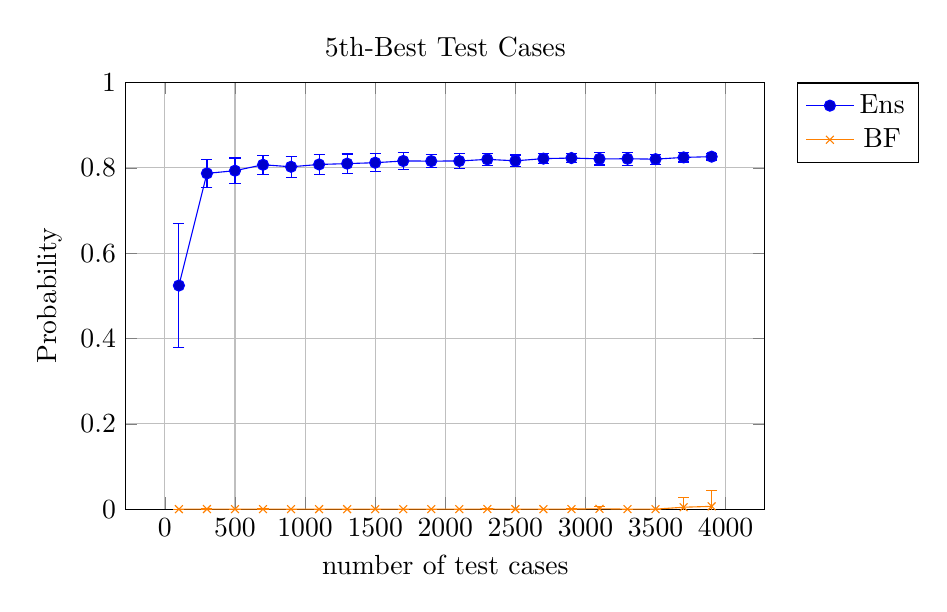
\begin{tikzpicture}
\begin{axis}[width=0.8\columnwidth,height=7cm,
  ymin=0,ymax=1,
  xtick={0,500,1000,1500,2000,2500,3000,3500,4000},
  xticklabels={0,500,1000,1500,2000,2500,3000,3500,4000},
  xlabel={number of test cases},ylabel={Probability},
  title={5th-Best Test Cases},grid=major,
  legend style={at={(1.05,1)},anchor=north west},
  error bars/y dir=both,error bars/y explicit]
\addplot+[mark=*,color=blue,error bars/.cd,y dir=both,y explicit] coordinates {
(100,0.5240999999999999) +- (0,0.1459288686102845)
(300,0.7869199999999996) +- (0,0.0323115193965602)
(500,0.7933000000000002) +- (0,0.02969384599198827)
(700,0.8071800000000002) +- (0,0.02274498374838471)
(900,0.8024400000000002) +- (0,0.025052728068485245)
(1100,0.8078800000000002) +- (0,0.02423325426443788)
(1300,0.80986) +- (0,0.022575957954226865)
(1500,0.812) +- (0,0.020587295468173485)
(1700,0.8160000000000001) +- (0,0.019509286119639493)
(1900,0.8157800000000001) +- (0,0.015060815491377126)
(2100,0.81598) +- (0,0.016939857600056826)
(2300,0.8198399999999999) +- (0,0.014676595278864616)
(2500,0.8164200000000001) +- (0,0.013618849482408164)
(2700,0.82156) +- (0,0.011609566779872795)
(2900,0.8228999999999997) +- (0,0.009998469270598465)
(3100,0.82098) +- (0,0.014304972733212695)
(3300,0.8212) +- (0,0.01566746270954878)
(3500,0.8202999999999996) +- (0,0.011714721246258934)
(3700,0.8244400000000001) +- (0,0.010766842525048061)
(3900,0.82616) +- (0,0.007926602072020715)
};
\addlegendentry{Ens}
\addplot+[mark=x,color=orange,error bars/.cd,y dir=both,y explicit] coordinates {
(100,0.0) +- (0,0.0)
(300,0.00021999999999999998) +- (0,0.0015556349186104045)
(500,0.0) +- (0,0.0)
(700,6e-05) +- (0,0.0004242640687119285)
(900,0.0) +- (0,0.0)
(1100,0.0) +- (0,0.0)
(1300,0.0) +- (0,0.0)
(1500,0.0) +- (0,0.0)
(1700,0.0) +- (0,0.0)
(1900,0.0) +- (0,0.0)
(2100,0.0) +- (0,0.0)
(2300,0.00028000000000000003) +- (0,0.001979898987322333)
(2500,0.0) +- (0,0.0)
(2700,2e-05) +- (0,0.0001414213562373095)
(2900,0.00012) +- (0,0.000848528137423857)
(3100,0.00078) +- (0,0.00551543289325507)
(3300,0.0) +- (0,0.0)
(3500,0.0) +- (0,0.0)
(3700,0.0044800000000000005) +- (0,0.022178533471327075)
(3900,0.00656) +- (0,0.03668239860405722)
};
\addlegendentry{BF}
\end{axis}
\end{tikzpicture}
\caption{RaceToWait (5th)}
\label{fig:RaceToWait_(5th)}
\end{figure}
\pgfplotsset{compat=1.3,width=0.8\columnwidth}
\begin{figure}[H]\centering\vspace{3ex}
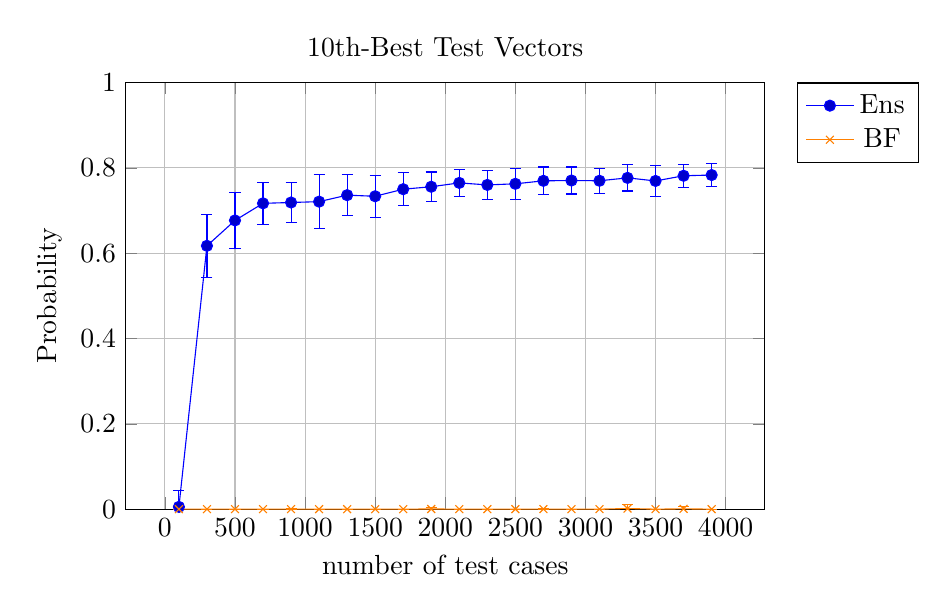
\begin{tikzpicture}
\begin{axis}[width=0.8\columnwidth,height=7cm,
  ymin=0,ymax=1,
  xtick={0,500,1000,1500,2000,2500,3000,3500,4000},
  xticklabels={0,500,1000,1500,2000,2500,3000,3500,4000},
  xlabel={number of test cases},ylabel={Probability},
  title={10th-Best Test Vectors},grid=major,
  legend style={at={(1.05,1)},anchor=north west},
  error bars/y dir=both,error bars/y explicit]
\addplot+[mark=*,color=blue,error bars/.cd,y dir=both,y explicit] coordinates {
(100,0.00532) +- (0,0.03761808075912433)
(300,0.6171999999999997) +- (0,0.07371068651235498)
(500,0.6766800000000001) +- (0,0.06483902830731453)
(700,0.7167800000000001) +- (0,0.04904320877074228)
(900,0.7187399999999998) +- (0,0.04589998443821709)
(1100,0.7207400000000002) +- (0,0.06308976759752888)
(1300,0.7359200000000001) +- (0,0.04865700025144777)
(1500,0.73332) +- (0,0.04885189612596467)
(1700,0.74992) +- (0,0.03831600081385514)
(1900,0.7556599999999999) +- (0,0.03456116140338779)
(2100,0.76468) +- (0,0.03184364864747247)
(2300,0.7599400000000002) +- (0,0.0337689689701377)
(2500,0.76252) +- (0,0.03674525653129969)
(2700,0.7695200000000003) +- (0,0.03238810565246296)
(2900,0.77028) +- (0,0.03162215704733837)
(3100,0.7696600000000002) +- (0,0.029494108716480862)
(3300,0.7764400000000002) +- (0,0.03086055536685983)
(3500,0.76926) +- (0,0.03620001691283853)
(3700,0.7814000000000001) +- (0,0.027069072645318888)
(3900,0.7830800000000001) +- (0,0.027380046361821793)
};
\addlegendentry{Ens}
\addplot+[mark=x,color=orange,error bars/.cd,y dir=both,y explicit] coordinates {
(100,0.0) +- (0,0.0)
(300,0.0) +- (0,0.0)
(500,0.0) +- (0,0.0)
(700,0.0) +- (0,0.0)
(900,0.0001) +- (0,0.0007071067811865476)
(1100,0.0) +- (0,0.0)
(1300,0.0) +- (0,0.0)
(1500,2e-05) +- (0,0.0001414213562373096)
(1700,0.0) +- (0,0.0)
(1900,0.0004) +- (0,0.0028284271247461905)
(2100,0.0) +- (0,0.0)
(2300,2e-05) +- (0,0.0001414213562373096)
(2500,0.0) +- (0,0.0)
(2700,0.0002) +- (0,0.0014142135623730952)
(2900,0.0) +- (0,0.0)
(3100,0.0) +- (0,0.0)
(3300,0.0014199999999999998) +- (0,0.010040916292848975)
(3500,0.0) +- (0,0.0)
(3700,0.00066) +- (0,0.004666904755831214)
(3900,0.0) +- (0,0.0)
};
\addlegendentry{BF}
\end{axis}
\end{tikzpicture}
\caption{RaceToWait (10th)}
\label{fig:RaceToWait_(10th)}
\end{figure}
%----------------------------------------

\pgfplotsset{compat=1.3,width=0.8\columnwidth}
\begin{figure}[H]\centering\vspace{3ex}
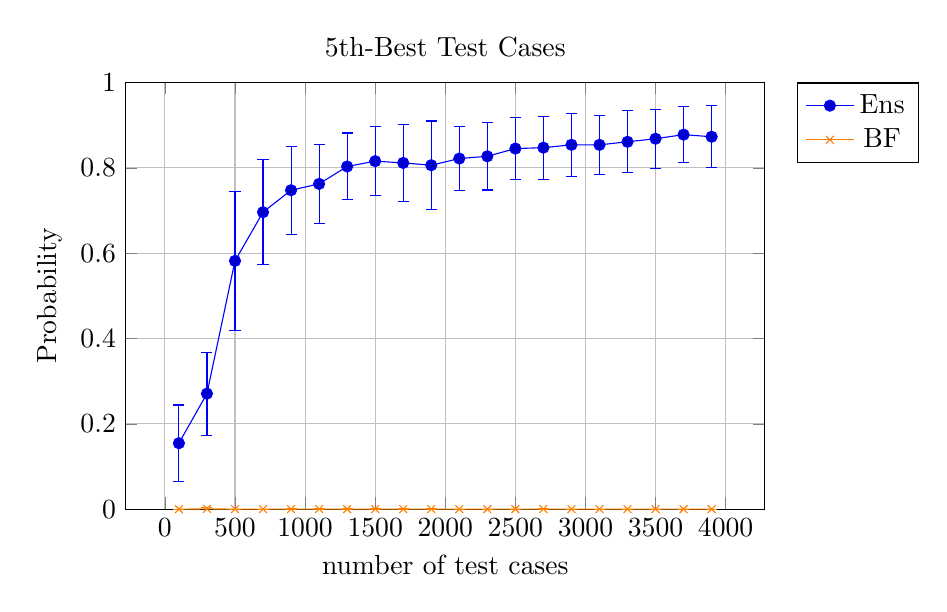
\begin{tikzpicture}
\begin{axis}[width=0.8\columnwidth,height=7cm,
  ymin=0,ymax=1,
  xtick={0,500,1000,1500,2000,2500,3000,3500,4000},
  xticklabels={0,500,1000,1500,2000,2500,3000,3500,4000},
  xlabel={number of test cases},ylabel={Probability},
  title={5th-Best Test Cases},grid=major,
  legend style={at={(1.05,1)},anchor=north west},
  error bars/y dir=both,error bars/y explicit]
\addplot+[mark=*,color=blue,error bars/.cd,y dir=both,y explicit] coordinates {
(100,0.15455999999999998) +- (0,0.08946237608455239)
(300,0.2707800000000001) +- (0,0.09720445316077693)
(500,0.5818599999999998) +- (0,0.162656644750938)
(700,0.69604) +- (0,0.12298895918590606)
(900,0.7474600000000001) +- (0,0.10341282634693436)
(1100,0.7623799999999998) +- (0,0.09314108017586395)
(1300,0.8031599999999999) +- (0,0.07841396168894353)
(1500,0.8155800000000002) +- (0,0.08143586182902918)
(1700,0.8114999999999999) +- (0,0.09050115570352411)
(1900,0.8061000000000001) +- (0,0.10368363380190396)
(2100,0.8217399999999998) +- (0,0.07522803700097729)
(2300,0.8270200000000003) +- (0,0.0788818517189616)
(2500,0.8451000000000002) +- (0,0.07271505753168829)
(2700,0.8472399999999999) +- (0,0.07404536943451545)
(2900,0.8539200000000001) +- (0,0.074078237736345)
(3100,0.8538200000000002) +- (0,0.06956561724042142)
(3300,0.8610200000000003) +- (0,0.07287828544769642)
(3500,0.8682399999999996) +- (0,0.0692895610125084)
(3700,0.87774) +- (0,0.06521293536389472)
(3900,0.8728) +- (0,0.07285574228345676)
};
\addlegendentry{Ens}
\addplot+[mark=x,color=orange,error bars/.cd,y dir=both,y explicit] coordinates {
(100,0.0) +- (0,0.0)
(300,0.00062) +- (0,0.0035160854857152067)
(500,0.0) +- (0,0.0)
(700,0.0) +- (0,0.0)
(900,6e-05) +- (0,0.0004242640687119285)
(1100,0.00021999999999999998) +- (0,0.0015556349186104045)
(1300,4e-05) +- (0,0.00019794866372215738)
(1500,8e-05) +- (0,0.000565685424949238)
(1700,6e-05) +- (0,0.0003136356914300021)
(1900,8e-05) +- (0,0.00039589732744431475)
(2100,0.0) +- (0,0.0)
(2300,2e-05) +- (0,0.00014142135623730954)
(2500,2e-05) +- (0,0.00014142135623730962)
(2700,0.00026) +- (0,0.0018384776310850235)
(2900,0.0) +- (0,0.0)
(3100,0.0) +- (0,0.0)
(3300,0.0) +- (0,0.0)
(3500,0.0) +- (0,0.0)
(3700,0.0) +- (0,0.0)
(3900,0.0) +- (0,0.0)
};
\addlegendentry{BF}
\end{axis}
\end{tikzpicture}
\caption{RacyIncrement (5th)}
\label{fig:RacyIncrement_(5th)}
\end{figure}
\pgfplotsset{compat=1.3,width=0.8\columnwidth}
\begin{figure}[H]\centering\vspace{3ex}
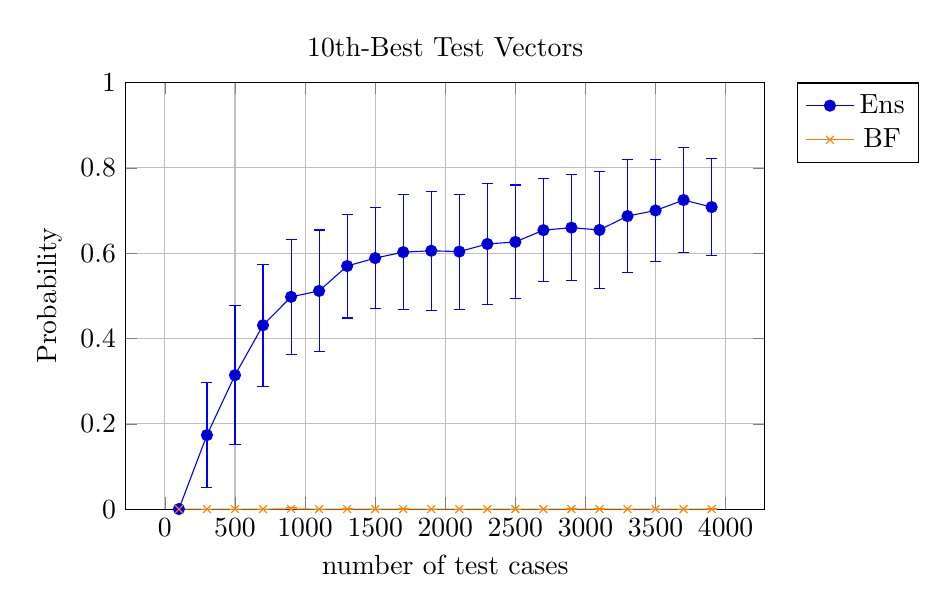
\begin{tikzpicture}
\begin{axis}[width=0.8\columnwidth,height=7cm,
  ymin=0,ymax=1,
  xtick={0,500,1000,1500,2000,2500,3000,3500,4000},
  xticklabels={0,500,1000,1500,2000,2500,3000,3500,4000},
  xlabel={number of test cases},ylabel={Probability},
  title={10th-Best Test Vectors},grid=major,
  legend style={at={(1.05,1)},anchor=north west},
  error bars/y dir=both,error bars/y explicit]
\addplot+[mark=*,color=blue,error bars/.cd,y dir=both,y explicit] coordinates {
(100,0.00028) +- (0,0.0014433521074645815)
(300,0.17364000000000004) +- (0,0.12391368951403066)
(500,0.31407999999999997) +- (0,0.16222708196367525)
(700,0.43108000000000013) +- (0,0.14304799251742464)
(900,0.49756000000000006) +- (0,0.1344192588242363)
(1100,0.5114599999999999) +- (0,0.1427985894288079)
(1300,0.5698199999999999) +- (0,0.12181529845949376)
(1500,0.58842) +- (0,0.11830694943964225)
(1700,0.60232) +- (0,0.13413265441193598)
(1900,0.6055799999999999) +- (0,0.1395848202377915)
(2100,0.6036199999999999) +- (0,0.1347384298921284)
(2300,0.6215399999999999) +- (0,0.1419708521392436)
(2500,0.62628) +- (0,0.13345472976990883)
(2700,0.6539) +- (0,0.12096503964504196)
(2900,0.6597799999999998) +- (0,0.12393831414976572)
(3100,0.6543800000000001) +- (0,0.1370693091476135)
(3300,0.6868999999999998) +- (0,0.13248168914677988)
(3500,0.7000399999999999) +- (0,0.11994368746735011)
(3700,0.7244999999999999) +- (0,0.12369436494184936)
(3900,0.7080199999999999) +- (0,0.11356064459133829)
};
\addlegendentry{Ens}
\addplot+[mark=x,color=orange,error bars/.cd,y dir=both,y explicit] coordinates {
(100,0.0) +- (0,0.0)
(300,0.0) +- (0,0.0)
(500,0.0) +- (0,0.0)
(700,2e-05) +- (0,0.0001414213562373095)
(900,0.00058) +- (0,0.0030107968976972976)
(1100,0.0) +- (0,0.0)
(1300,0.00017999999999999998) +- (0,0.0012727922061357855)
(1500,0.0) +- (0,0.0)
(1700,4e-05) +- (0,0.000282842712474619)
(1900,0.0) +- (0,0.0)
(2100,0.0) +- (0,0.0)
(2300,2e-05) +- (0,0.00014142135623730954)
(2500,2e-05) +- (0,0.0001414213562373096)
(2700,0.0) +- (0,0.0)
(2900,0.00014000000000000001) +- (0,0.0009899494936611666)
(3100,8e-05) +- (0,0.000565685424949238)
(3300,0.0) +- (0,0.0)
(3500,0.0) +- (0,0.0)
(3700,0.0) +- (0,0.0)
(3900,0.00012) +- (0,0.000848528137423857)
};
\addlegendentry{BF}
\end{axis}
\end{tikzpicture}
\caption{RacyIncrement (10th)}
\label{fig:RacyIncrement_(10th)}
\end{figure}
%----------------------------------------

\pgfplotsset{compat=1.3,width=0.8\columnwidth}
\begin{figure}[H]\centering\vspace{3ex}
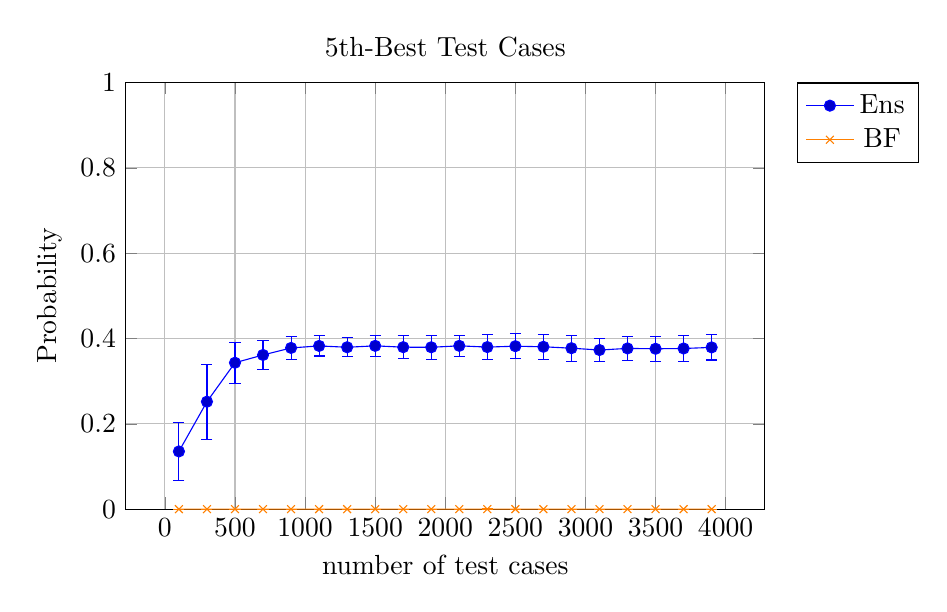
\begin{tikzpicture}
\begin{axis}[width=0.8\columnwidth,height=7cm,
  ymin=0,ymax=1,
  xtick={0,500,1000,1500,2000,2500,3000,3500,4000},
  xticklabels={0,500,1000,1500,2000,2500,3000,3500,4000},
  xlabel={number of test cases},ylabel={Probability},
  title={5th-Best Test Cases},grid=major,
  legend style={at={(1.05,1)},anchor=north west},
  error bars/y dir=both,error bars/y explicit]
\addplot+[mark=*,color=blue,error bars/.cd,y dir=both,y explicit] coordinates {
(100,0.13526) +- (0,0.06862462519878312)
(300,0.25187999999999994) +- (0,0.08792660204362969)
(500,0.34313999999999995) +- (0,0.048080718694754866)
(700,0.36135999999999996) +- (0,0.03408438507766349)
(900,0.3778600000000001) +- (0,0.026261642704732323)
(1100,0.3825800000000001) +- (0,0.023669570579724748)
(1300,0.3794400000000001) +- (0,0.022539000213235835)
(1500,0.38273999999999986) +- (0,0.02441713182440993)
(1700,0.37964) +- (0,0.027098279183259542)
(1900,0.3793800000000001) +- (0,0.028242311577937565)
(2100,0.38277999999999984) +- (0,0.025244348731095104)
(2300,0.37982) +- (0,0.02904583991428946)
(2500,0.38192) +- (0,0.029238526443229464)
(2700,0.38056000000000006) +- (0,0.028851597769925172)
(2900,0.37724) +- (0,0.03052436965536132)
(3100,0.37294000000000005) +- (0,0.02685213479143033)
(3300,0.3767400000000002) +- (0,0.02823791777026061)
(3500,0.3758799999999999) +- (0,0.02928859916104433)
(3700,0.37656) +- (0,0.03037262462367407)
(3900,0.3791) +- (0,0.029493167662621635)
};
\addlegendentry{Ens}
\addplot+[mark=x,color=orange,error bars/.cd,y dir=both,y explicit] coordinates {
(100,0.0) +- (0,0.0)
(300,0.0) +- (0,0.0)
(500,0.0) +- (0,0.0)
(700,0.0) +- (0,0.0)
(900,0.0) +- (0,0.0)
(1100,0.0) +- (0,0.0)
(1300,0.0) +- (0,0.0)
(1500,0.0) +- (0,0.0)
(1700,0.0) +- (0,0.0)
(1900,0.0) +- (0,0.0)
(2100,0.0) +- (0,0.0)
(2300,4e-05) +- (0,0.000282842712474619)
(2500,0.0) +- (0,0.0)
(2700,0.0) +- (0,0.0)
(2900,0.0) +- (0,0.0)
(3100,0.0) +- (0,0.0)
(3300,0.0) +- (0,0.0)
(3500,0.0) +- (0,0.0)
(3700,0.0) +- (0,0.0)
(3900,0.0) +- (0,0.0)
};
\addlegendentry{BF}
\end{axis}
\end{tikzpicture}
\caption{SemaphoreLeak (5th)}
\label{fig:SemaphoreLeak_(5th)}
\end{figure}
\pgfplotsset{compat=1.3,width=0.8\columnwidth}
\begin{figure}[H]\centering\vspace{3ex}
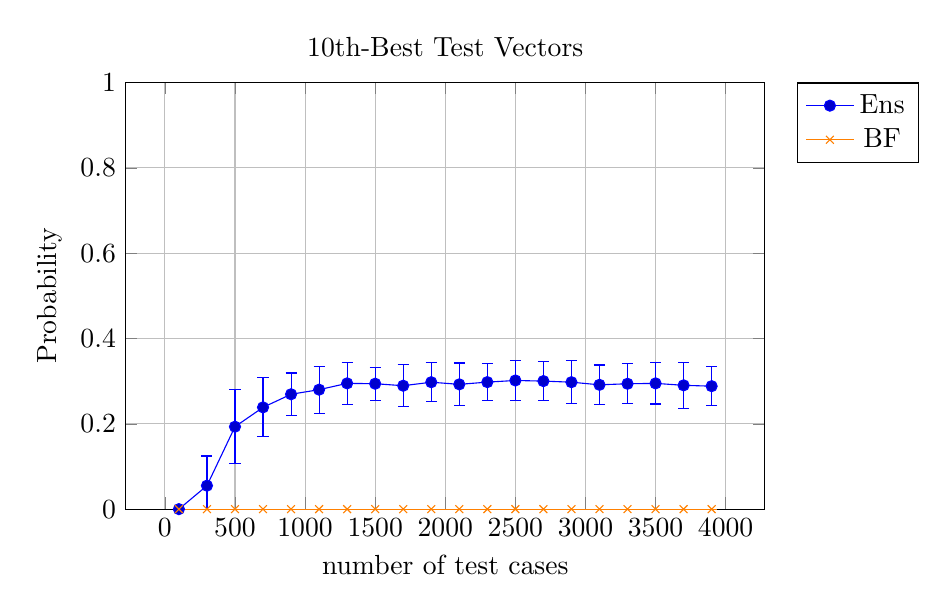
\begin{tikzpicture}
\begin{axis}[width=0.8\columnwidth,height=7cm,
  ymin=0,ymax=1,
  xtick={0,500,1000,1500,2000,2500,3000,3500,4000},
  xticklabels={0,500,1000,1500,2000,2500,3000,3500,4000},
  xlabel={number of test cases},ylabel={Probability},
  title={10th-Best Test Vectors},grid=major,
  legend style={at={(1.05,1)},anchor=north west},
  error bars/y dir=both,error bars/y explicit]
\addplot+[mark=*,color=blue,error bars/.cd,y dir=both,y explicit] coordinates {
(100,0.0) +- (0,0.0)
(300,0.055020000000000006) +- (0,0.06953709625158384)
(500,0.19322) +- (0,0.08651159884485944)
(700,0.23855999999999994) +- (0,0.06911840181447892)
(900,0.26928) +- (0,0.04987946287127113)
(1100,0.28003999999999996) +- (0,0.05532241675775178)
(1300,0.2948200000000001) +- (0,0.048747868608560584)
(1500,0.29400000000000004) +- (0,0.038923263071885796)
(1700,0.28929999999999995) +- (0,0.04880124203839312)
(1900,0.2975000000000001) +- (0,0.04597348392812651)
(2100,0.2925000000000001) +- (0,0.0500731098148552)
(2300,0.29772000000000004) +- (0,0.04303631119917921)
(2500,0.30156000000000005) +- (0,0.04592636519917625)
(2700,0.30012000000000005) +- (0,0.04571903546753335)
(2900,0.29756000000000005) +- (0,0.05086001597020716)
(3100,0.29142) +- (0,0.04638133421178485)
(3300,0.2938599999999999) +- (0,0.04668348045014256)
(3500,0.29480000000000006) +- (0,0.048444792900616256)
(3700,0.2902000000000001) +- (0,0.053500715234585265)
(3900,0.28824) +- (0,0.045670318141914475)
};
\addlegendentry{Ens}
\addplot+[mark=x,color=orange,error bars/.cd,y dir=both,y explicit] coordinates {
(100,0.0) +- (0,0.0)
(300,0.0) +- (0,0.0)
(500,0.0) +- (0,0.0)
(700,0.0) +- (0,0.0)
(900,0.0) +- (0,0.0)
(1100,0.0) +- (0,0.0)
(1300,0.0) +- (0,0.0)
(1500,0.0) +- (0,0.0)
(1700,0.0) +- (0,0.0)
(1900,0.0) +- (0,0.0)
(2100,0.0) +- (0,0.0)
(2300,0.0) +- (0,0.0)
(2500,0.0) +- (0,0.0)
(2700,0.0) +- (0,0.0)
(2900,0.0) +- (0,0.0)
(3100,0.0) +- (0,0.0)
(3300,0.0) +- (0,0.0)
(3500,0.0) +- (0,0.0)
(3700,0.0) +- (0,0.0)
(3900,0.0) +- (0,0.0)
};
\addlegendentry{BF}
\end{axis}
\end{tikzpicture}
\caption{SemaphoreLeak (10th)}
\label{fig:SemaphoreLeak_(10th)}
\end{figure}
%----------------------------------------

\pgfplotsset{compat=1.3,width=0.8\columnwidth}
\begin{figure}[H]\centering\vspace{3ex}
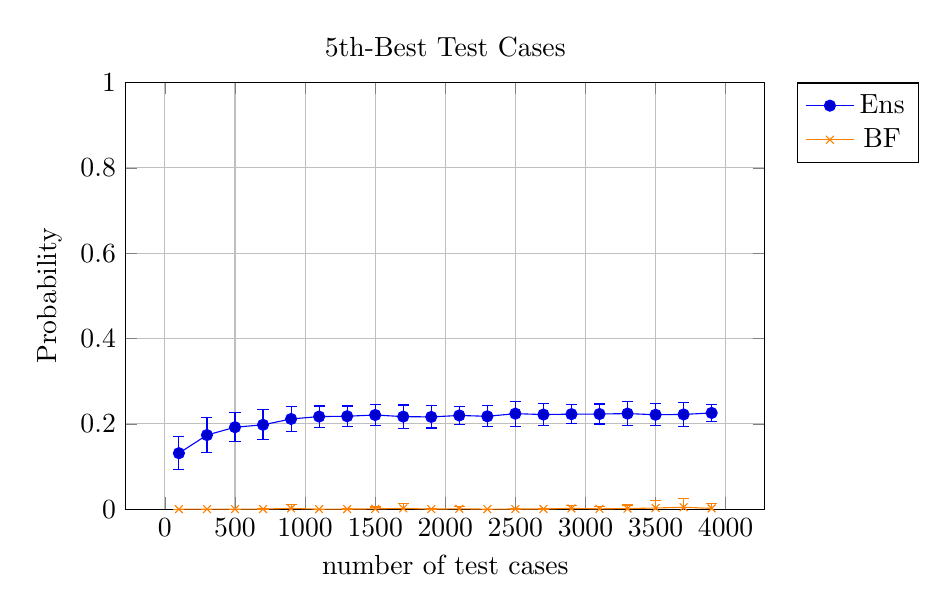
\begin{tikzpicture}
\begin{axis}[width=0.8\columnwidth,height=7cm,
  ymin=0,ymax=1,
  xtick={0,500,1000,1500,2000,2500,3000,3500,4000},
  xticklabels={0,500,1000,1500,2000,2500,3000,3500,4000},
  xlabel={number of test cases},ylabel={Probability},
  title={5th-Best Test Cases},grid=major,
  legend style={at={(1.05,1)},anchor=north west},
  error bars/y dir=both,error bars/y explicit]
\addplot+[mark=*,color=blue,error bars/.cd,y dir=both,y explicit] coordinates {
(100,0.13113999999999998) +- (0,0.03921682791655571)
(300,0.17362) +- (0,0.04182318954447961)
(500,0.19204000000000002) +- (0,0.033772927208711105)
(700,0.19763999999999993) +- (0,0.03533730179228785)
(900,0.21136) +- (0,0.028473947992607464)
(1100,0.21694000000000002) +- (0,0.02471916549677877)
(1300,0.21777999999999995) +- (0,0.02403508489942299)
(1500,0.22064000000000003) +- (0,0.02416166638394326)
(1700,0.21686) +- (0,0.027250171315694616)
(1900,0.21616) +- (0,0.02591773484685411)
(2100,0.21960000000000002) +- (0,0.021795899258571456)
(2300,0.2175800000000001) +- (0,0.024783215188953777)
(2500,0.22382) +- (0,0.02920769398215321)
(2700,0.2217000000000001) +- (0,0.02582772596593459)
(2900,0.22264000000000003) +- (0,0.022815819789195512)
(3100,0.22292) +- (0,0.023464989117528222)
(3300,0.22399999999999995) +- (0,0.02735704960819676)
(3500,0.22125999999999998) +- (0,0.025817103965062895)
(3700,0.22196000000000002) +- (0,0.027657497046138298)
(3900,0.22548000000000004) +- (0,0.020397318751367736)
};
\addlegendentry{Ens}
\addplot+[mark=x,color=orange,error bars/.cd,y dir=both,y explicit] coordinates {
(100,0.0) +- (0,0.0)
(300,2e-05) +- (0,0.00014142135623730956)
(500,2e-05) +- (0,0.00014142135623730954)
(700,0.0002) +- (0,0.0014142135623730952)
(900,0.00168) +- (0,0.008920144594783021)
(1100,0.0) +- (0,0.0)
(1300,0.00014000000000000001) +- (0,0.0005717856027482714)
(1500,0.00062) +- (0,0.0043840620433565946)
(1700,0.0017000000000000001) +- (0,0.011735607772753757)
(1900,6e-05) +- (0,0.0004242640687119285)
(2100,0.0007599999999999999) +- (0,0.005374011537017761)
(2300,0.0) +- (0,0.0)
(2500,0.0003) +- (0,0.0021213203435596424)
(2700,0.00048) +- (0,0.0019403344967256736)
(2900,0.0017000000000000001) +- (0,0.006421424598759299)
(3100,0.00068) +- (0,0.004808326112068524)
(3300,0.0013999999999999998) +- (0,0.00841281820819169)
(3500,0.00264) +- (0,0.01852385114452418)
(3700,0.0044800000000000005) +- (0,0.02053890285804587)
(3900,0.0017599999999999998) +- (0,0.012445079348883236)
};
\addlegendentry{BF}
\end{axis}
\end{tikzpicture}
\caption{SharedCounter (5th)}
\label{fig:SharedCounter_(5th)}
\end{figure}
\pgfplotsset{compat=1.3,width=0.8\columnwidth}
\begin{figure}[H]\centering\vspace{3ex}
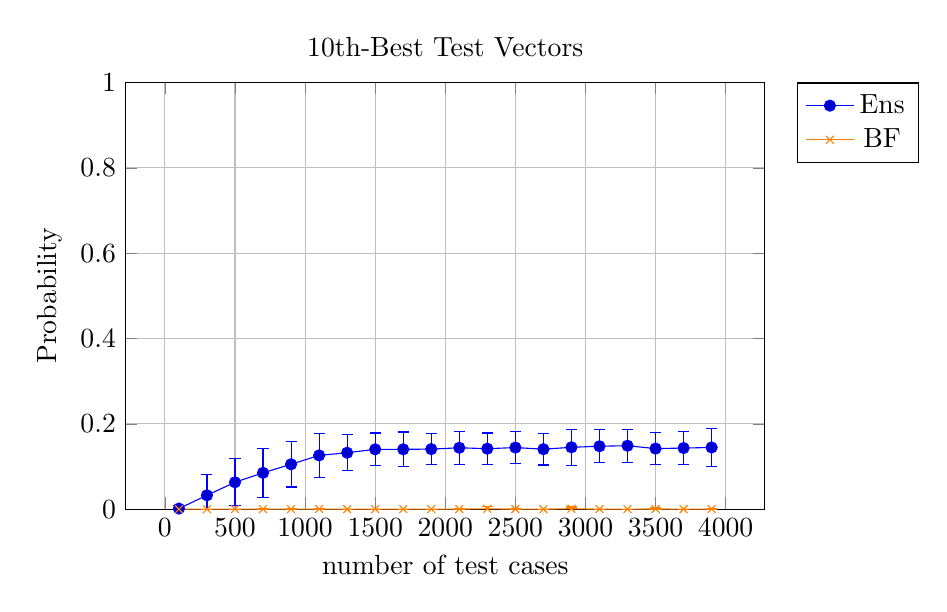
\begin{tikzpicture}
\begin{axis}[width=0.8\columnwidth,height=7cm,
  ymin=0,ymax=1,
  xtick={0,500,1000,1500,2000,2500,3000,3500,4000},
  xticklabels={0,500,1000,1500,2000,2500,3000,3500,4000},
  xlabel={number of test cases},ylabel={Probability},
  title={10th-Best Test Vectors},grid=major,
  legend style={at={(1.05,1)},anchor=north west},
  error bars/y dir=both,error bars/y explicit]
\addplot+[mark=*,color=blue,error bars/.cd,y dir=both,y explicit] coordinates {
(100,0.00136) +- (0,0.006156993700546674)
(300,0.03246) +- (0,0.049259914572332225)
(500,0.06298000000000001) +- (0,0.05472994553967242)
(700,0.08511999999999997) +- (0,0.057301437101328914)
(900,0.10517999999999997) +- (0,0.053321776383900614)
(1100,0.12596) +- (0,0.05086033697834705)
(1300,0.13224) +- (0,0.04167687167546372)
(1500,0.1402) +- (0,0.03825958596701421)
(1700,0.14022) +- (0,0.0406208401323904)
(1900,0.14070000000000005) +- (0,0.03556095657674371)
(2100,0.14382) +- (0,0.038652660494011455)
(2300,0.1417) +- (0,0.03681462109720282)
(2500,0.14433999999999997) +- (0,0.03765450348435178)
(2700,0.14048000000000002) +- (0,0.036940791015032705)
(2900,0.14498000000000003) +- (0,0.0420415198078648)
(3100,0.14744) +- (0,0.038227119340348344)
(3300,0.14866000000000001) +- (0,0.038890537120886116)
(3500,0.14190000000000003) +- (0,0.0374537810412476)
(3700,0.14318) +- (0,0.03888008251439969)
(3900,0.14456000000000002) +- (0,0.04368307008721902)
};
\addlegendentry{Ens}
\addplot+[mark=x,color=orange,error bars/.cd,y dir=both,y explicit] coordinates {
(100,0.0) +- (0,0.0)
(300,0.0) +- (0,0.0)
(500,0.0) +- (0,0.0)
(700,4e-05) +- (0,0.000282842712474619)
(900,4e-05) +- (0,0.0001979486637221573)
(1100,0.00021999999999999998) +- (0,0.001298193407181295)
(1300,0.0) +- (0,0.0)
(1500,0.0) +- (0,0.0)
(1700,2e-05) +- (0,0.00014142135623730954)
(1900,2e-05) +- (0,0.00014142135623730954)
(2100,0.00021999999999999998) +- (0,0.0012001700559776127)
(2300,0.00084) +- (0,0.0059396969619669995)
(2500,8e-05) +- (0,0.000565685424949238)
(2700,0.0) +- (0,0.0)
(2900,0.00102) +- (0,0.003997397112305631)
(3100,0.0) +- (0,0.0)
(3300,0.0) +- (0,0.0)
(3500,0.00041999999999999996) +- (0,0.002268596617348465)
(3700,0.0) +- (0,0.0)
(3900,0.00026) +- (0,0.0015754494013856903)
};
\addlegendentry{BF}
\end{axis}
\end{tikzpicture}
\caption{SharedCounter (10th)}
\label{fig:SharedCounter_(10th)}
\end{figure}
%----------------------------------------

\pgfplotsset{compat=1.3,width=0.8\columnwidth}
\begin{figure}[H]\centering\vspace{3ex}
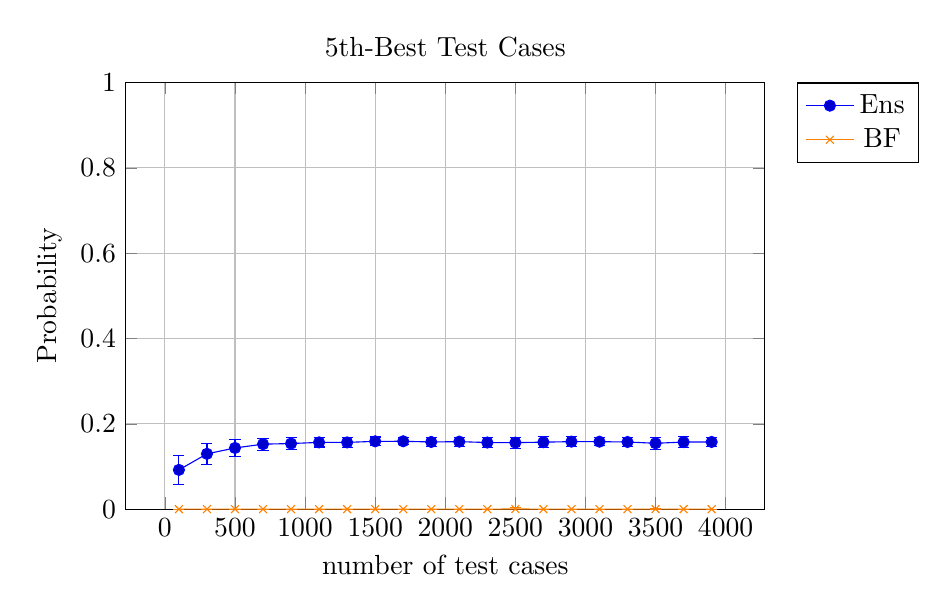
\begin{tikzpicture}
\begin{axis}[width=0.8\columnwidth,height=7cm,
  ymin=0,ymax=1,
  xtick={0,500,1000,1500,2000,2500,3000,3500,4000},
  xticklabels={0,500,1000,1500,2000,2500,3000,3500,4000},
  xlabel={number of test cases},ylabel={Probability},
  title={5th-Best Test Cases},grid=major,
  legend style={at={(1.05,1)},anchor=north west},
  error bars/y dir=both,error bars/y explicit]
\addplot+[mark=*,color=blue,error bars/.cd,y dir=both,y explicit] coordinates {
(100,0.092) +- (0,0.03469576225372989)
(300,0.12964000000000003) +- (0,0.0251686231613239)
(500,0.14340000000000003) +- (0,0.019280951792917472)
(700,0.15233999999999992) +- (0,0.014040190126045668)
(900,0.15376) +- (0,0.013325684881124135)
(1100,0.15648) +- (0,0.010740425256658958)
(1300,0.15646) +- (0,0.01199695539607905)
(1500,0.15889999999999996) +- (0,0.010164463907684078)
(1700,0.15905999999999998) +- (0,0.008546177090204887)
(1900,0.15745999999999996) +- (0,0.0111469040270272)
(2100,0.15822) +- (0,0.010710075363213572)
(2300,0.15611999999999998) +- (0,0.011005824061164442)
(2500,0.15589999999999996) +- (0,0.013012160717214194)
(2700,0.15699999999999997) +- (0,0.01224078162103538)
(2900,0.15823999999999996) +- (0,0.011523817394723797)
(3100,0.15815999999999994) +- (0,0.009721341975052542)
(3300,0.15737999999999996) +- (0,0.011424802950116015)
(3500,0.15437999999999993) +- (0,0.013761659249746098)
(3700,0.15721999999999994) +- (0,0.013725129641408472)
(3900,0.15749999999999997) +- (0,0.010554523162306933)
};
\addlegendentry{Ens}
\addplot+[mark=x,color=orange,error bars/.cd,y dir=both,y explicit] coordinates {
(100,0.0) +- (0,0.0)
(300,0.0) +- (0,0.0)
(500,0.0) +- (0,0.0)
(700,0.0) +- (0,0.0)
(900,0.0) +- (0,0.0)
(1100,0.0) +- (0,0.0)
(1300,0.0) +- (0,0.0)
(1500,0.0) +- (0,0.0)
(1700,0.0) +- (0,0.0)
(1900,0.0) +- (0,0.0)
(2100,0.0) +- (0,0.0)
(2300,0.0) +- (0,0.0)
(2500,0.00042) +- (0,0.0029698484809834997)
(2700,0.0) +- (0,0.0)
(2900,0.0) +- (0,0.0)
(3100,0.0) +- (0,0.0)
(3300,0.0) +- (0,0.0)
(3500,0.00016) +- (0,0.001131370849898476)
(3700,0.0) +- (0,0.0)
(3900,0.0) +- (0,0.0)
};
\addlegendentry{BF}
\end{axis}
\end{tikzpicture}
\caption{SharedFlag (5th)}
\label{fig:SharedFlag_(5th)}
\end{figure}
\pgfplotsset{compat=1.3,width=0.8\columnwidth}
\begin{figure}[H]\centering\vspace{3ex}
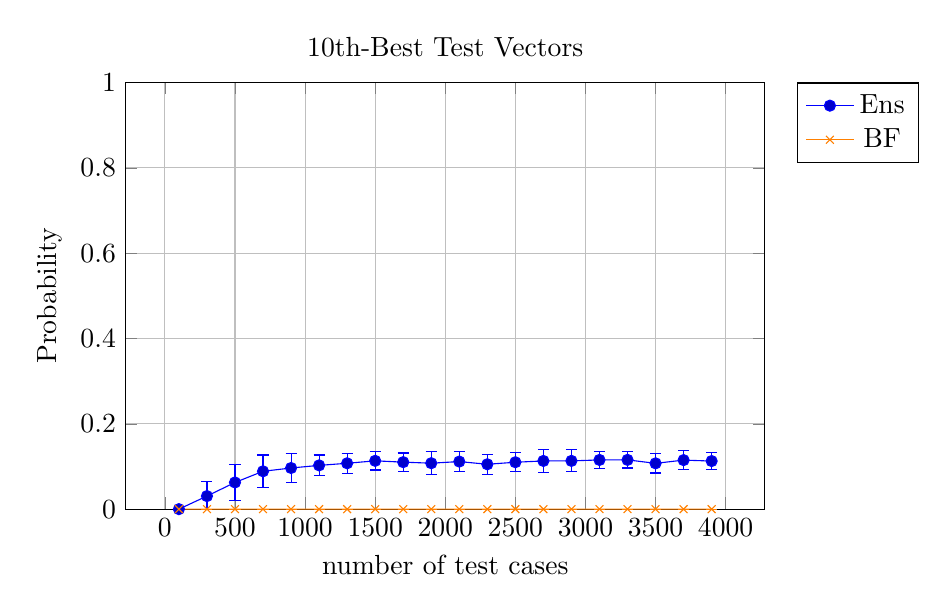
\begin{tikzpicture}
\begin{axis}[width=0.8\columnwidth,height=7cm,
  ymin=0,ymax=1,
  xtick={0,500,1000,1500,2000,2500,3000,3500,4000},
  xticklabels={0,500,1000,1500,2000,2500,3000,3500,4000},
  xlabel={number of test cases},ylabel={Probability},
  title={10th-Best Test Vectors},grid=major,
  legend style={at={(1.05,1)},anchor=north west},
  error bars/y dir=both,error bars/y explicit]
\addplot+[mark=*,color=blue,error bars/.cd,y dir=both,y explicit] coordinates {
(100,0.0) +- (0,0.0)
(300,0.03064) +- (0,0.03433553523089216)
(500,0.06255999999999999) +- (0,0.041521157626109716)
(700,0.08870000000000003) +- (0,0.038322077613995024)
(900,0.09644000000000004) +- (0,0.03367986135993557)
(1100,0.10258000000000005) +- (0,0.02437553976377751)
(1300,0.10748) +- (0,0.023042321311633716)
(1500,0.11324000000000002) +- (0,0.02158756255677913)
(1700,0.11015999999999998) +- (0,0.021549525303735374)
(1900,0.10770000000000005) +- (0,0.026560865796067822)
(2100,0.11150000000000002) +- (0,0.022752662997314894)
(2300,0.10516000000000002) +- (0,0.023199542571141353)
(2500,0.10994000000000004) +- (0,0.022569990912623593)
(2700,0.11298000000000002) +- (0,0.026246469150290386)
(2900,0.11312) +- (0,0.02582408304869943)
(3100,0.11536000000000003) +- (0,0.02074112546884274)
(3300,0.11548) +- (0,0.018999720728344868)
(3500,0.10735999999999997) +- (0,0.022544975457235567)
(3700,0.11494000000000003) +- (0,0.02209941360381864)
(3900,0.11268000000000006) +- (0,0.019982073598756072)
};
\addlegendentry{Ens}
\addplot+[mark=x,color=orange,error bars/.cd,y dir=both,y explicit] coordinates {
(100,0.0) +- (0,0.0)
(300,0.0) +- (0,0.0)
(500,0.0) +- (0,0.0)
(700,0.0) +- (0,0.0)
(900,2e-05) +- (0,0.0001414213562373096)
(1100,0.0) +- (0,0.0)
(1300,0.0) +- (0,0.0)
(1500,0.0) +- (0,0.0)
(1700,0.0) +- (0,0.0)
(1900,0.0) +- (0,0.0)
(2100,0.0) +- (0,0.0)
(2300,0.0) +- (0,0.0)
(2500,0.0) +- (0,0.0)
(2700,0.0) +- (0,0.0)
(2900,2e-05) +- (0,0.0001414213562373095)
(3100,0.0) +- (0,0.0)
(3300,0.0) +- (0,0.0)
(3500,0.0) +- (0,0.0)
(3700,0.0) +- (0,0.0)
(3900,0.0) +- (0,0.0)
};
\addlegendentry{BF}
\end{axis}
\end{tikzpicture}
\caption{SharedFlag (10th)}
\label{fig:SharedFlag_(10th)}
\end{figure}
%----------------------------------------
